\documentclass{amsart}[12pt]
\usepackage{graphicx}
\usepackage{comment}
\usepackage{amscd,mathabx}
\usepackage{amssymb,setspace}
\usepackage{tikz-cd}
\usepackage{latexsym,amsfonts,amssymb,amsthm,amsmath,amscd,stmaryrd,mathrsfs,xcolor}
\usepackage[all, knot]{xy}
\usepackage[top=1in, bottom=1in, left=1in, right=1in]{geometry}
\xyoption{all}
\xyoption{arc}
\usepackage{hyperref}


\newcommand{\qbox}{\tag*{$\blacksquare$}}
%\usepackage[notcite,notref]{showkeys}
 
%\CompileMatricesx
\newcommand{\edit}[1]{\marginpar{\footnotesize{#1}}}
%\newcommand{\edit}[1]{}
\newcommand{\rperf}[2]{\operatorname{RPerf}(#1 \into #2)}



\newcommand{\vectwo}[2]{\begin{bmatrix} #1 \\ #2 \end{bmatrix}}

\newcommand{\vecfour}[4]{\begin{bmatrix} #1 \\ #2 \\ #3 \\ #4 \end{bmatrix}}

\newcommand{\Cat}[1]{\left<\left< \text{#1} \right>\right>}


\def\htpy{\simeq_{\mathrm{htpc}}}
\def\tor{\text{ or }}
\def\fg{finitely generated~}

\def\Ass{\operatorname{Ass}}
\def\ann{\operatorname{ann}}
\def\inc{\operatorname{inc}}
\def\Der{\operatorname{Der}}

\newcommand{\Tor}{\mathrm{Tor}}
\newcommand{\can}{\mathrm{can}}

\def\ob{{\mathfrak{ob}} }
\def\BiAdd{\operatorname{BiAdd}}
\def\BiLin{\operatorname{BiLin}}

\def\Syl{\operatorname{Syl}}
\def\span{\operatorname{span}}

\def\sdp{\rtimes}
\def\cL{\mathcal L}
\def\cR{\mathcal R}



\def\ay{??}
\def\Aut{\operatorname{Aut}}
\def\End{\operatorname{End}}
\def\Mat{\operatorname{Mat}}


\def\a{\alpha}



\def\etale{\'etale~}
\def\tW{\tilde{W}}
\def\tH{\tilde{H}}
\def\tC{\tilde{C}}
\def\tS{\tilde{S}}
\def\tX{\tilde{X}}
\def\tZ{\tilde{Z}}
\def\HBM{H^{\text{BM}}}
\def\tHBM{\tilde{H}^{\text{BM}}}
\def\Hc{H_{\text{c}}}
\def\Hs{H_{\text{sing}}}
\def\cHs{{\mathcal H}_{\text{sing}}}
\def\sing{{\text{sing}}}
\def\Hms{H^{\text{sing}}}
\def\Hm{\Hms}
\def\tHms{\tilde{H}^{\text{sing}}}
\def\Grass{\operatorname{Grass}}
\def\image{\operatorname{im}}
\def\im{\image}
\def\ker{\operatorname{ker}}
\def\coker{\operatorname{coker}}
\def\cone{\operatorname{cone}}
\newcommand{\Hom}{\mathrm{Hom}}
\newcommand{\Spec}{\mathrm{Spec}}

\newcommand{\onto}{\twoheadrightarrow}


\def\ku{ku}
\def\bbu{\bf bu}
\def\KR{K{\mathbb R}}

\def\CW{\underline{CW}}
\def\cP{\mathcal P}
\def\cE{\mathcal E}
\def\cL{\mathcal L}
\def\cJ{\mathcal J}
\def\cJmor{\cJ^\mor}
\def\ctJ{\tilde{\mathcal J}}
\def\tPhi{\tilde{\Phi}}
\def\cA{\mathcal A}
\def\cB{\mathcal B}
\def\cC{\mathcal C}
\def\cZ{\mathcal Z}
\def\cD{\mathcal D}
\def\cF{\mathcal F}
\def\cG{\mathcal G}
\def\cO{\mathcal O}
%\def\cI{\mathcal I}
\def\cS{\mathcal S}
\def\cT{\mathcal T}
\def\cM{\mathcal M}
\def\cN{\mathcal N}
\def\cMpc{{\mathcal M}_{pc}}
\def\cMpctf{{\mathcal M}_{pctf}}
\def\L{\Lambda}

\def\sA{\mathscr A}
\def\sB{\mathscr B}
\def\sC{\mathscr C}
\def\sZ{\mathscr  Z}
\def\sD{\mathscr  D}
\def\sF{\mathscr  F}
\def\sG{\mathscr G}
\def\sO{\mathscr  O}
\def\sI{\mathscr I}
\def\sS{\mathscr S}
\def\sT{\mathscr  T}
\def\sM{\mathscr M}
\def\sN{\mathscr N}

%\newcommand{\inc}{\subseteq}
\newcommand{\id}{\mathrm{id}}


\newcommand{\Jan}[1]{\textcolor{violet}{Lecture of January #1, 2023}}
\newcommand{\Feb}[1]{\textcolor{violet}{Lecture of February #1, 2023}}
\newcommand{\Mar}[1]{\textcolor{violet}{Lecture of March #1, 2023}}
\newcommand{\Apr}[1]{\textcolor{violet}{Lecture of April #1, 2023}}
\newcommand{\May}[1]{\textcolor{violet}{Lecture of May #1, 2023}}

\def\Ext{\operatorname{Ext}}
 \def\ext{\operatorname{ext}}



\def\ov#1{{\overline{#1}}}

\def\vecthree#1#2#3{\begin{bmatrix} #1 \\ #2 \\ #3 \end{bmatrix}}

\def\tOmega{\tilde{\Omega}}
\def\tDelta{\tilde{\Delta}}
\def\tSigma{\tilde{\Sigma}}
\def\tsigma{\tilde{\sigma}}


\newcommand{\bs}[1]{\mathbf{#1}}

\def\d{\delta}
\def\td{\tilde{\delta}}

\def\e{\epsilon}
\def\nsg{\unlhd}
\def\pnsg{\lhd}

\newcommand{\tensor}{\otimes}
\newcommand{\homotopic}{\simeq}
\newcommand{\homeq}{\cong}
\newcommand{\iso}{\approx}

\DeclareMathOperator{\ho}{Ho}
\DeclareMathOperator*{\colim}{colim}


\newcommand{\Q}{\mathbb{Q}}
\renewcommand{\H}{\mathbb{H}}

\newcommand{\bP}{\mathbb{P}}
\newcommand{\bM}{\mathbb{M}}
\newcommand{\A}{\mathbb{A}}
\newcommand{\bH}{{\mathbb{H}}}
\newcommand{\G}{\mathbb{G}}
\newcommand{\bR}{{\mathbb{R}}}
\newcommand{\bL}{{\mathbb{L}}}
\newcommand{\R}{{\mathbb{R}}}
\newcommand{\F}{\mathbb{F}}
\newcommand{\E}{\mathbb{E}}
\newcommand{\bF}{\mathbb{F}}
\newcommand{\bE}{\mathbb{E}}
\newcommand{\bK}{\mathbb{K}}


\newcommand{\bD}{\mathbb{D}}
\newcommand{\bS}{\mathbb{S}}

\newcommand{\bN}{\mathbb{N}}


\newcommand{\bG}{\mathbb{G}}

\newcommand{\C}{\mathbb{C}}
\newcommand{\Z}{\mathbb{Z}}
\newcommand{\N}{\mathbb{N}}

\newcommand{\M}{\mathcal{M}}
\newcommand{\W}{\mathcal{W}}



\newcommand{\itilde}{\tilde{\imath}}
\newcommand{\jtilde}{\tilde{\jmath}}
\newcommand{\ihat}{\hat{\imath}}
\newcommand{\jhat}{\hat{\jmath}}

\newcommand{\fc}{{\mathfrak c}}
\newcommand{\fp}{{\mathfrak p}}
\newcommand{\fm}{{\mathfrak m}}
\newcommand{\fn}{{\mathfrak n}}
\newcommand{\fq}{{\mathfrak q}}

\newcommand{\op}{\mathrm{op}}
\newcommand{\dual}{\vee}

\newcommand{\DEF}[1]{\emph{#1}\index{#1}}
\newcommand{\Def}[1]{#1 \index{#1}}


% The following causes equations to be numbered within sections
\numberwithin{equation}{section}


\theoremstyle{plain} %% This is the default, anyway
\newtheorem{thm}[equation]{Theorem}
\newtheorem{thmdef}[equation]{TheoremDefinition}
\newtheorem{introthm}{Theorem}
\newtheorem{introcor}[introthm]{Corollary}
\newtheorem*{introthm*}{Theorem}
\newtheorem{question}{Question}
\newtheorem{cor}[equation]{Corollary}
\newtheorem{por}[equation]{Porism}
\newtheorem{lem}[equation]{Lemma}
\newtheorem{lemminition}[equation]{Lemminition}
\newtheorem{prop}[equation]{Proposition}
\newtheorem{porism}[equation]{Porism}
\newtheorem{fact}[equation]{Fact}


\newtheorem{conj}[equation]{Conjecture}
\newtheorem{quest}[equation]{Question}

\theoremstyle{definition}
\newtheorem{defn}[equation]{Definition}
\newtheorem{chunk}[equation]{}
\newtheorem{ex}[equation]{Example}

\newtheorem{exer}[equation]{Optional Exercise}

\theoremstyle{remark}
\newtheorem{rem}[equation]{Remark}

\newtheorem{notation}[equation]{Notation}
\newtheorem{terminology}[equation]{Terminology}



\renewcommand{\sec}[1]{\section{#1}}
\newcommand{\ssec}[1]{\subsection{#1}}
\newcommand{\sssec}[1]{\subsubsection{#1}}

\newcommand{\br}[1]{\lbrace \, #1 \, \rbrace}
\newcommand{\li}{ < \infty}
\newcommand{\quis}{\simeq}
\newcommand{\xra}[1]{\xrightarrow{#1}}
\newcommand{\xla}[1]{\xleftarrow{#1}}
\newcommand{\xlra}[1]{\overset{#1}{\longleftrightarrow}}

\newcommand{\xroa}[1]{\overset{#1}{\twoheadrightarrow}}
\newcommand{\xria}[1]{\overset{#1}{\hookrightarrow}}
\newcommand{\ps}[1]{\mathbb{P}_{#1}^{\text{c}-1}}




\def\and{{ \text{ and } }}
\def\oor{{ \text{ or } }}

\def\Perm{\operatorname{Perm}}
\newcommand{\Ss}{\mathbb{S}}

\def\Op{\operatorname{Op}}
\def\res{\operatorname{res}}
\def\ind{\operatorname{ind}}

\def\sign{{\mathrm{sign}}}
\def\naive{{\mathrm{naive}}}
\def\l{\lambda}


\def\ov#1{\overline{#1}}
\def\cV{{\mathcal V}}
%%%-------------------------------------------------------------------
%%%-------------------------------------------------------------------

\newcommand{\chara}{\operatorname{char}}
\newcommand{\Kos}{\operatorname{Kos}}
\newcommand{\opp}{\operatorname{opp}}
\newcommand{\perf}{\operatorname{perf}}

\newcommand{\Fun}{\operatorname{Fun}}
\newcommand{\GL}{\operatorname{GL}}
\newcommand{\SL}{\operatorname{SL}}
\def\o{\omega}
\def\oo{\overline{\omega}}

\def\cont{\operatorname{cont}}
\def\te{\tilde{e}}
\def\gcd{\operatorname{gcd}}

\def\stab{\operatorname{stab}}

\def\va{\underline{a}}

\def\ua{\underline{a}}
\def\ub{\underline{b}}


\newcommand{\Ob}{\mathrm{Ob}}
\newcommand{\Set}{\mathbf{Set}}
\newcommand{\Grp}{\mathbf{Grp}}
\newcommand{\Ab}{\mathbf{Ab}}
\newcommand{\Sgrp}{\mathbf{Sgrp}}
\newcommand{\Ring}{\mathbf{Ring}}
\newcommand{\Fld}{\mathbf{Fld}}
\newcommand{\cRing}{\mathbf{cRing}}
\newcommand{\Mod}[1]{#1-\mathbf{Mod}}
\newcommand{\Cx}[1]{#1-\mathbf{Comp}}
\newcommand{\vs}[1]{#1-\mathbf{vect}}
\newcommand{\Vs}[1]{#1-\mathbf{Vect}}
\newcommand{\vsp}[1]{#1-\mathbf{vect}^+}
\newcommand{\Top}{\mathbf{Top}}
\newcommand{\Setp}{\mathbf{Set}_*}
\newcommand{\Alg}[1]{#1-\mathbf{Alg}}
\newcommand{\cAlg}[1]{#1-\mathbf{cAlg}}
\newcommand{\PO}{\mathbf{PO}}
\newcommand{\Cont}{\mathrm{Cont}}
\newcommand{\MaT}[1]{\mathbf{Mat}_{#1}}
\newcommand{\Rep}[2]{\mathbf{Rep}_{#1}(#2)}
\newcommand{\Holo}{\mathrm{Holo}}

\newcommand{\red}[1]{{\color{red}#1}}
\newcommand{\blue}[1]{{\color{blue}#1}}

%%%-------------------------------------------------------------------
%%%-------------------------------------------------------------------
%%%-------------------------------------------------------------------
%%%-------------------------------------------------------------------
%%%-------------------------------------------------------------------

\makeindex
\title{Math 918 Lecture Notes, Spring 2023}


\begin{document}
\onehalfspacing

\maketitle

%\tableofcontents

\Jan{24}

\sec{Derivations}

\ssec{Definition and first examples}

Our goal will be to consider derivatives algebraically.

The usual notion of derivative of a function is a rule that turns certain real-valued or complex-valued functions into other real-valued or complex-valued functions as follows: at a given point $x$, we take
\[ f'(x) = \lim_{y\to x} \frac{f(y)-f(x)}{y-x}.\]
This certainly gives us derivative functions on some rings, for example,
the ring of infinitely-differentiable functions on $\R$:\index{infinitely-differentiable functions on $\R$}\index{$\cC^{\infty}(\R)$}
\[  \cC^{\infty}(\R) \xra{\frac{d}{dx}} \cC^{\infty}(\R)\]
or the ring of \emph{entire functions}\index{entire}, i.e., \emph{holomorphic}\index{holomorphic}, a.k.a. complex-differentiable, functions on the complex plane\index{$\Holo(\C)$}:
\[ \Holo(\C) \xra{\frac{d}{dx}}\Holo(\C). \]
Neither of these is the sort of ring that we usually consider in commutative algebra. In particular, neither is Noetherian.

Using our familiar rules of differentiation, we might recall that the derivative of a polynomial is a polynomial, and the derivative of a rational function is a rational function. So, we get derivatives on much more manageable rings:
\[ \R[x] \xra{\frac{d}{dx}} \R[x], \quad \R(x) \xra{\frac{d}{dx}} \R(x), \quad \C[x] \xra{\frac{d}{dx}} \C[x], \quad \C(x) \xra{\frac{d}{dx}} \C(x).\]

To unlock some of the applications of derivatives, we would like to be able to do this as much as possible over arbitrary rings. We might be optimistic about doing this for arbitrary polynomial rings at least, given the examples above. To do it, we certainly must get rid of this limit approach, since moving around in fields like $\Q$ or $\F_p$ we certainly will miss out on lots of limits. Of course, when we actually compute the derivative of a real or complex polynomial, we don't consider the limit definition anymore, but instead use rules of derivative. Namely, we have a sum rule, a scalar rule, a product rule, a quotient rule, and a power rule, and knowing all of these, we easily and limitlessly compute derivatives of any polynomial or rational function over $\R$ or $\C$. Since the quotient rule and power rule (mostly) follow from the product rule, we will hone in on the first three for our definition of algebraic notion of derivative.

So, our first approximation of the definition of \emph{derivation}, our notion of derivative, is a function $\partial$ from a ring $R$ to itself that satisfies a sum rule, a scalar rule, and a product rule:
\begin{itemize}
\item $\partial(r+s) = \partial(r)+\partial(s)$ for all $r,s\in R$,
\item $\partial(cr)= c\partial(r)$ for all $r\in R$ and $c$ ``constant???",
\item $\partial(rs) = r\partial(s) + s\partial(r)$ for all $r,s\in R$.
\end{itemize}

There is something we must change (``constant???") and something else less clear we can/should change. Let's be openminded. If $R$ is a ring, let's let our constants be any reasonable set of elements of $R$: any subring $A$ of $R$. But let's be even more openminded. Look at the right-hand sides above. To make sense of them we have to be able to add our outputs together and multiply them by ring elements, but we don't have to multiply them with each other. They don't have to live in $R$---they just have to live in an $R$-module.

\begin{defn} Let $R$ be a ring and $M$ be an $R$-module. A \emph{derivation}\index{derivation} from $R$ to $M$ is a function $\partial:R\to M$ such that
\begin{itemize}
\item $\partial(r+s) = \partial(r) + \partial(s)$ for all $r,s\in R$,
\item $\partial(rs) = r\partial(s) + s\partial(r)$ for all $r,s\in R$.
\end{itemize}
If $R$ is an $A$-algebra, then $\partial$ is a \emph{derivation over $A$}\index{derivation over $A$} or an \emph{$A$-linear derivation}\index{$A$-linear derivation} if in addition
\begin{itemize}
\item $\partial(ar) = a \partial(r)$ for all $a\in A$ and $r\in R$.
\end{itemize}
\end{defn}



\begin{rem} Recall that $R$ is an $A$-algebra means that $R$ is equipped with a ring homomorphism $\phi:A\to R$. In this case, every $R$-module is also an $A$-module by restriction of scalars: $a  m := \phi(a) m$; i.e., for $A$ to act on $M$, just view elements of $A$ as elements of $R$ via $\phi$ and do the same action. This is what's going on in the right-hand side above. We'll circle back to restriction of scalars soon.
\end{rem}

\sssec{Examples of derivations}

Let's consider some examples of derivations to buy into this notion. 


First, let's construct the ``usual derivative'' for a polynomial or a power series ring, and show it is a derivation.

\begin{defn}
Let $A$ be a ring and $R=A[x]$ a polynomial ring. We define $\frac{d}{dx}:R\to R$ by the rule
\[ \frac{d}{dx} ( \sum_{j=0}^d a_j x^j) = \sum_{j=1}^d j a_j x^{j-1}.\]\index{$\frac{d}{dx}$}
Similarly, for a power series ring, $R= A\llbracket x\rrbracket$, we define
$\frac{d}{dx}:R\to R$ by the rule
\[ \frac{d}{dx} ( \sum_{j=0}^\infty a_j x^j) = \sum_{j=1}^\infty j a_j x^{j-1}.\]
\end{defn}


\begin{lem}
The functions $\frac{d}{dx}: A[x] \to A[x]$ and $\frac{d}{dx}: A\llbracket x\rrbracket \to  A\llbracket x\rrbracket$ are $A$-linear derivations.
\end{lem}
\begin{proof}
In either case, we have a well-defined function returning an object of the same type. The formulas are the same in both cases, just allowing infinite formal sums for power series, so we'll deal with both simultaneously. 

Take $r= \sum_{j=0} a_j x^j$, $s= \sum_{j=0} b_j x^j$, and $c$ with $a_j,b_j,c\in A$. Then
\[ \frac{d}{dx} (r+s) = \frac{d}{dx}  (\sum_{j=0} (a_j+b_j) x^j ) = \sum_{j=1} j (a_j+b_j) x^{j-1} = \frac{d}{dx}(r) + \frac{d}{dx}(s),\]
\[ \frac{d}{dx} (cr) = \frac{d}{dx}  (\sum_{j=0} (ca_j) x^j ) = \sum_{j=1} j (ca_j) x^{j-1} = c \frac{d}{dx}(r) ,\]
and
\[\begin{aligned}
 r\frac{d}{dx}(s) + s \frac{d}{dx}(r) &= (\sum_{i=0} a_i x^i )( \sum_{j=1} j b_j x^{j-1}) + (\sum_{j=0} b_j x^j )( \sum_{i=1} i a_i x^{i-1}) 
 \\ &= \sum_{k=1} \sum_{i+j=k} (a_i j b_j) x^{i+j-1} + \sum_{k=1} \sum_{i+j=k} (i a_i b_j) x^{i+j-1} 
 \\&= \sum_{k=1} \sum_{i+j=k} k a_i b_j x^{i+j-1} 
 \\&= \frac{d}{dx}  (\sum_{k=0} \sum_{i+j=k} (a_ib_j) x^k ) = \frac{d}{dx} (rs). \qedhere
\end{aligned}\]
 \end{proof}
 


 
 Note that we could have written the formula above as $\frac{d}{dx} ( \sum_{j=0}^d a_j x^j) = \sum_{j=1}^d j a_j x^{j-1}$ as well: it looks like we have something illegal when $j=0$, but the coefficient of zero tells us to ignore it.

\begin{prop}
Let $A$ be a ring, $\{X_\lambda \  | \ \lambda\in \Lambda\}$, and $R=A[X_\lambda \  | \ \lambda\in \Lambda]$ be a polynomial ring. Then the partial derivatives $\frac{d}{d X_\lambda}$ given by the rule
\[ \frac{d}{dx_\lambda} ( \sum_{\alpha} a_\alpha X^{\alpha}) = \sum_{\alpha} \alpha_\lambda a_\alpha X^{\alpha-e_\lambda}\]\index{$\frac{d}{dx_\lambda}$}where $\alpha\in \N^{\Lambda}$ is an exponent tuple and $e_\lambda$ is the unit vector in the $\lambda$ coordinate,
are $A$-linear derivations. Similarly for the power series ring $R=A\llbracket X_\lambda \  | \ \lambda\in \Lambda\rrbracket$.
\end{prop}
\begin{proof}
Consider $R$ as $R'[X_\lambda]$, with $R'=A[X_\mu \ | \ \mu\in \Lambda\smallsetminus \{\lambda\}]$. Then $\frac{d}{d X_\lambda}$ is just the ``usual derivative'' in this polynomial ring over $R'$, so it is an $R'$-linear derivation of $R$. But since $A\subseteq R'$, this is an $A$-linear derivation as well.
\end{proof}



So we can differentiate over any polynomial ring now, e.g., over $R=\F_2[x]$. Let's not neglect our original derivatives.

\begin{ex}
The standard derivatives
\[  \cC^{\infty}(\R) \xra{\frac{d}{dx}} \cC^{\infty}(\R)\]
and 
\[ \Holo(\C) \xra{\frac{d}{dx}}\Holo(\C) \]
are $\R$-linear and $\C$-linear derivations, respectively.
\end{ex}

We haven't seen examples where we take derivations into ``actual'' modules yet. It turns out that this is a natural thing to do. In fact, examples like this appear in calculus before derivations back into the ring!

\begin{ex}
Let's return to old-fashioned derivatives of $\C^\infty$ functions. Before we get derivatives of functions as functions, we start with the notion of derivative at a point, which should just be a number. Let's try to realize ``derivative at $x=x_0$'' for some real number $x_0$, which we'll write as $\frac{d}{dx}|_{x=x_0}$\index{derivative at $x=x_0$}\index{$\frac{d}{dx}|_{x=x_0}$}, as a derivation on $\cC^{\infty}(\R)$. The target should be $\R$:
\[ \frac{d}{dx}|_{x=x_0} : \cC^{\infty}(\R) \to \R,\]
so we need to view $\R$ as a $\cC^{\infty}(\R)$-module. A very $x=x_0$ flavored way of doing so is by the rule
\[ f \cdot c = f(x_0) c.\]
Another useful way of thinking about this module structure is as the quotient $\cC^{\infty}(\R)/\fm_{x_0}$, where $\fm_{x_0}$ is the maximal ideal consisting of functions with $f(x_0)=0$. Indeed, the evaluation at $0$ map
\[ \mathrm{ev}_{x_0}  \cC^{\infty}(\R) \to \R\]
has kernel $\fm_{x_0}$ by definition, and if $\R$ has the module structure given above, this map is $\cC^{\infty}(\R)$-linear: if $f\in  \cC^{\infty}(\R)$ and $c\in \R$, then $\mathrm{ev}_{x_0}(fc) = f(x_0) c = f\cdot c$. Of course, if $x_0$ changed, we would get a different module structure.

Back to our derivative. Take $f,g\in \cC^{\infty}(\R)$ and $c\in \R$. Note that this $c$ is an element of $\R \subseteq \cC^{\infty}(\R)$ as opposed to $\R\cong \cC^{\infty}(\R)/\fm_{x_0}$. Then
\[  \frac{d}{dx}|_{x=x_0}\ (f+g) = \frac{d}{dx}|_{x=x_0}\ f + \frac{d}{dx}|_{x=x_0} \ g\]
\[ \frac{d}{dx}|_{x=x_0}\ cf = c \frac{d}{dx}|_{x=x_0}\ f \]
and by the product rule
\[ \frac{d}{dx}|_{x=x_0}\ (fg) =  f(x_0) (\frac{d}{dx}|_{x=x_0} \ g) +  g(x_0) (\frac{d}{dx}|_{x=x_0} \ f) = f \cdot  (\frac{d}{dx}|_{x=x_0}\ g) + g \cdot (\frac{d}{dx}|_{x=x_0}\ f).\]
\end{ex}

\Jan{26}

\begin{ex}
Other natural uses of derivatives actually take values in modules rather than the ring itself.
Let's consider $R=\cC^\infty(\R^3)$, the ring of infinitely differentiable real valued functions from $\R^3$ to $\R$, with pointwise operations. One has a notion of gradient $\nabla$ of a function:
\[ f(x,y,z) \mapsto \begin{bmatrix} \frac{\partial f}{\partial x} & \frac{\partial f}{\partial y} & \frac{\partial f}{\partial z} \end{bmatrix}.\]
The output is a vector of three functions in $R$, so this is a function $\nabla:R\to R^3$.
It follows from calculus that this is an $\R$-linear derivation.

Similarly, one sometimes talks about the \emph{total derivative}\index{total derivative} of a function $f\in \cC^\infty(\R^3)$ as
\[ df = \frac{\partial f}{\partial x} dx + \frac{\partial f}{\partial y} dy + \frac{\partial f}{\partial z} dz.\]
This rule $f\mapsto df$ is a derivation from $R$ to a free $R$-module with basis $dx,dy,dz$.
\end{ex}



\begin{ex} Let's try out a slightly more interesting ring. Let's consider $R=\C[x,y]/(x^2-y^3)$ and try out $\frac{d}{dx}$ on this ring. Of course, this is a quotient ring, so if this means anything, 
it means apply this rule to an equivalence class and take the class of the result. But this is a problem, since $0 = x^2+y^3$ and $\frac{d}{dx}(0) = 0 \neq 2x = \frac{d}{dx}(x^2+y^3)$. So this 
derivation doesn't even make sense, and in hindsight, perhaps it looks a little bit silly to try. 
But we can actually get by with something surprisingly similar. Let's write $\frac{d}{dx}|_{(0,0)}$ for the rule
\[ \frac{d}{dx}|_{(0,0)} (f) = \frac{d}{dx}(f) (0,0);\]
i.e., partial derivative with respect to $x$ at the origin. It is in fact well-defined:
we have 
\[\begin{aligned}
\frac{d}{dx}|_{(0,0)} (f+(x^2+y^3)g) &= \frac{d}{dx}|_{(0,0)} (f) + \frac{d}{dx}|_{(0,0)} ((x^2+y^3)g) 
\\&=  \frac{d}{dx}|_{(0,0)} (f) + g|_{(0,0)} \frac{d}{dx}|_{(0,0)} (x^2+y^3) + (x^2+y^3)|_{(0,0)}  \frac{d}{dx}|_{(0,0)} (g) = \frac{d}{dx}|_{(0,0)} (f)\end{aligned}\]
and, along the same lines as previous examples, is a $\C$-linear derivation to $\C$, viewed as a module via the rule $f\cdot c= f(0,0) c$.
\end{ex}


\begin{ex} Let's end with a boring example. For any $A$-algebra $R$ and any $R$-module $M$, the zero map is an $A$-linear derivation from $R$ to $M$.
\end{ex}




\ssec{Properties of derivations}

Let's collect some basic properties of derivations. The first includes the fact that constants go to zero.

\begin{prop} Let $\partial:R\to M$ be a derivation.
\begin{enumerate}
\item $\partial(0)=\partial(1)=0$,
\item $\partial(-r) = -\partial(r)$,
\item The kernel of $\partial$ is a subring of $R$,
\item For $A\subseteq R$, $\partial$ is $A$-linear if and only if $A\subseteq \ker(\partial)$.
\end{enumerate}
\end{prop}
\begin{proof} 
\begin{enumerate}
\item $\partial(0) = \partial(0+0) = \partial(0) +\partial(0)$, and
$\partial(1)=\partial(1\cdot 1) = 1 \partial(1) + 1 \partial(1) = \partial(1) +\partial(1)$; in each case we cancel.
\item $0=\partial(r-r)= \partial(r) + \partial(-r)$, and move $\partial(r)$ to the other side.
\item If $\partial(r) = \partial(s)=0$, then $\partial(r-s) = \partial(r) - \partial(s) = 0$ and $\partial(rs) = r\partial(s) + s\partial(r)=0$.
\item If $A\subseteq \ker(\partial)$, $a\in A$, and $r\in R$, then $\partial(ar) = a \partial(r) + r\partial(a)= a\partial(r)$, so $\partial$ is $A$-linear; conversely, if $\partial(ar) = a \partial(r)$ for all $a\in A$ and $r\in R$, then $r\partial(a) = 0$ for all $a\in A$ and $r\in R$, and in particular $\partial(a)=1\partial(a)=0$.\qedhere
\end{enumerate}
\end{proof}

\begin{rem} It follows that every derivation of $R$ into $M$ is $\Z$-linear since every derivation is linear over its kernel, and its kernel is a subring.
\end{rem}

There are lots of ways to make derivations out of other derivations.

\begin{prop} Let $\alpha,\beta:R\to M$ be derivations over $A$, $t\in R$, and $\gamma:M\to N$ be an $R$-module homomorphism, and $\phi:S\to R$ an $A$-algebra homomorphism.
\begin{enumerate}
\item $\alpha+\beta:R\to M$ is a derivation over $A$,
\item $t\alpha:R\to M$ is a derivation over $A$,
\item $\gamma\circ \alpha:R\to N$ is a derivation over $A$.
\item $\alpha\circ \phi:S\to M$ is a derivation over $A$.
\end{enumerate}
\end{prop}
\begin{proof} In each case, the map under consideration is definitely $A$-linear, so we just need to check the product rule.
\begin{enumerate}
\item $(\alpha+\beta)(rs) =\alpha(rs) + \beta(rs) = r\alpha(s) + s\alpha(r) + r\beta(s)+s\beta(r) =r(\alpha+\beta)(s) + s(\alpha+\beta)(r)$;
\item $t\alpha(rs) = t(r\alpha(s) + s\alpha(r)) = r(t\alpha(s)) + s(t\alpha(r))$;
\item $(\gamma\circ \alpha)(rs)= \gamma((r\alpha(s) + s\alpha(r))= r\gamma\circ\alpha(s) + s\gamma\circ\alpha(r)$.
\item $(\alpha\circ \phi)(rs) = \alpha( \phi(r) \phi(s) ) = \phi(s) \alpha(\phi(r)) + \phi(r) \alpha(\phi(s)) = s (\alpha\circ \phi)(r) + r (\alpha\circ \phi)(s)$, where the last equality is just recalling that $M$ is a module by restriction of scalars.
\qedhere
\end{enumerate}
\end{proof}

\begin{defn} Let $R$ be a ring, and $M$ be and $R$-module. We set $\Der_R(M)$\index{$\Der_R(M)$} to be the \emph{module of derivations} of $R$ into $M$. If $R$ is an $A$-algebra via $\phi:R\to M$, we set $\Der_{R|A}(M)$\index{$\Der_{R|A}(M)$} or $\Der_\phi(M)$\index{$\Der_\phi(M)$} to be the \emph{module of $A$-linear derivations} of $R$ into $M$.
\end{defn}

These are $R$-modules as a consequence of the proposition above.

\begin{ex}
If $A$ is a ring and $R=A[x_1,\dots,x_n]$ is a polynomial ring over $A$, then for any $f_1,\dots,f_n\in R$,
\[\xymatrix@R=0pc@C=0pc{ \sum_{i=1}^n f_i \frac{d}{dx_i}:& R \ar[rrr] &&& R \\
& r \ar@{|->}[rrr] &&& \sum_{i=1}^n f_i \frac{dr}{dx_i}}\]
is an $A$-linear derivation on $R$.

If $M$ is an $R$-module, then for any $m_1,\dots,m_n \in M$, the map
\[ \xymatrix@R=0pc@C=0pc{m_i \frac{d}{dx_i}:& R\ar[rrr] &&& M\\
& r \ar@{|->}[rrr] &&& \frac{dr}{dx_i} m_i}\]
is an $A$-linear derivation, since it is the composition of the derivation $R\xra{\frac{d}{dx_i}} R$ and the $R$-linear map $R\xra{m} M$; adding these, the map
\[\xymatrix@R=0pc@C=0pc{ \sum_{i=1}^n m_i \frac{d}{dx_i}:& R \ar[rrr] &&& M \\
& r \ar@{|->}[rrr]&&& \sum_{i=1}^n \frac{dr}{dx_i} m_i}\]
is an $A$-linear derivation.
\end{ex}

\begin{ex}
Let's jack this example up.
Let $A$ be a ring, $R=A[X_\lambda \ | \ \lambda\in\Lambda]$ a polynomial ring over $A$, and $\{f_\lambda \ | \ \lambda\in \Lambda\}$ a sequence of elements in bijection with the variables
then the formal sum
\[ \sum_{\lambda\in \Lambda} f_\lambda \frac{d}{dX_\lambda} : R\to R\]
given by $r \mapsto \sum_{\lambda\in\Lambda} f_\lambda \frac{dr}{dX_\lambda}$
gives a well-defined map, since any $r\in R$ involves at most finitely many variables, and hence $ \frac{dr}{dX_\lambda}=0$ for all but finitely many $\lambda\in \Lambda$. This map is an $A$-linear derivation. Indeed, $A$-linearity is striaghtforward. To check the product rule, take $r,s\in R$; between the two, they involve only finitely many variables, and for these elements, the formula for this derivation agrees with the rule for the finitely many variables involved. By the last example, the product rule holds. 

Similarly, for any $R$-module $M$ and $\Lambda$-tuple of elements of $M$, there is a derivation
\[ \sum_{\lambda\in \Lambda} m_\lambda \frac{d}{dX_\lambda} : R\to M\]
given by $f \mapsto \sum_{\lambda\in \Lambda}  \frac{d}{dX_\lambda} m_\lambda$.
\end{ex}

We would like to compute modules of derivations in some examples. The following lemma will help us recognize when we're done.

\begin{lem} Let $R$ be an $A$-algebra and $\{f_\lambda \ | \ \lambda\in \Lambda\}$ be a generating set of $R$ as an $A$-algebra. Let $M$ be an $R$-module.
Then any $A$-linear derivation on $R$ is determined by the images of $f_\lambda$. That is, $\alpha,\beta:R\to M$ are $A$-linear derivations with $\alpha(f_\lambda) = \beta(f_\lambda)$ for all $\lambda$, then $\alpha=\beta$.
\end{lem}
\begin{proof} We need to show that $\alpha(r)=\beta(r)$ for any $r\in R$. Any element of $R$ can be written as a sum of monomial expressions in the $f's$; i.e., a sum of terms of the form $r=a f_{\lambda_1}^{\mu_1}\cdots f_{\lambda_n}^{\mu_n}$ with $a\in A$ so it suffices to show that $\alpha$ and $\beta$ take e same value on such a monomial $r$. We proceed by induction on $k=\mu_1+\cdots + \mu_n$. When $k=0$, $r\in A$ so $\alpha(r)=0=\beta(r)$. For the inductive step, take $k>0$, so WLOG $\mu_1\neq 0$; then $r= r' f_{\lambda_1}$, and
\[ \alpha(r' f_{\lambda_1}) = r' \alpha(f_{\lambda_1}) + f_{\lambda_1} \alpha(r')\]
and likewise for $\beta$. By the starting assumption, $\alpha(f_{\lambda_1}) = \beta(f_{\lambda_1})$ and by the induction hypothesis $\alpha(r')=\beta(r')$. The equality follows.
\end{proof}

\begin{thm}
Let $A$ be a ring and $R=A[X_\lambda \ | \ \lambda\in\Lambda]$ be a polynomial ring over $A$. For any $R$-module $M$, the map
\[\xymatrix@R=0pc{ \prod_{\Lambda} M \ar[r]^-{\mu} & \Der_{R|A}(M) \\ 
(m_\lambda)_\lambda \ar@{|->}[r] &  \sum m_\lambda \frac{d}{dX_\lambda}
}\]
is an isomorphism.
\end{thm}
\begin{proof}
Consider the map $\nu:\Der_{R|A}(M) \to \prod_{\Lambda} M$ given by $\alpha\mapsto (\alpha(X_\lambda))_{\lambda\in \Lambda}$. The previous lemma shows that $\nu$ is injective. On the other hand, 
\[ (\nu \circ \mu)(m_\lambda)_\lambda = ( (\sum_\lambda m_\lambda \frac{d}{dX_\lambda})(X_\lambda) )_\lambda = (m_\lambda)_\lambda.\]
Thus, $\mu$ is injective. Then $\mu$ must be an isomorphism. Indeed, $\nu = (\nu  \mu) \nu = \nu (\mu \nu)$ and $\nu$ injective implies $\mu \nu$ is the identity as well.
\end{proof}

\Jan{31}

We can give a description the derivations on any ring now.

\begin{prop} Let $R$ be an $A$-algebra. Write $R=S/I$ with $S=A[X_\lambda \ | \ \lambda\in \Lambda]$ and $I=(f_\gamma \ | \ \gamma\in\Gamma)$. Let $M$ be an $R$-module. Then every $A$-linear derivation $\partial$ from  $R$ to $M$ can be written in the form
\[ \xymatrix@R=0pc{ \sum_{\lambda\in \Lambda} m_\lambda \overline{\frac{d}{dx_{\lambda}}} \\
r = [ s] \mapsto  \sum_\lambda \frac{d}{dx_{\lambda}}(s) m_\lambda}\]
for some unique $(m_{\lambda})_\lambda \in \prod_{\Lambda} M$.
A tuple of elements $(m_\lambda)_\lambda$ induces a well-defined derivation from $R$ to $M$ if and only if the corresponding derivation $\widetilde{\partial}:S\to M$ has $\widetilde{\partial}(f_\gamma)=0$ for all $\gamma$.
\end{prop}
\begin{proof}
Let $\pi:S\to R$ be the quotient map. Given an $A$-linear derivation $\partial:R\to M$, there is an $A$-linear derivation $\pi\circ \partial:S\to M$ that can be written in the form above by the previous theorem, so any derivation has this form. Since derivations are addition, such a derivation is well-defined so long as $\widetilde{\partial}(I)=0$. This certainly implies that $\widetilde{\partial}(f_\gamma)=0$ for all $\gamma$; conversely, any element of $I$ can be written as $\sum_i s_i f_i$ and $\widetilde{\partial} (\sum_i s_i f_i) =\sum_i s_i \widetilde{\partial}(f_i) + \sum_i f_i \widetilde{\partial}(s_i)$, and the first sum is zero by hypothesis and the second since $M$ is an $R$-module which is necessarily killed by $I$.
\end{proof}

\begin{ex} Let's find some $\C$-linear derivations on $R=\frac{\C[x,y]}{x^2+y^3}$ to itself. Any such derivation must be a map of the form $\partial = r_1 \overline{\frac{d}{dx}} + r_2 \overline{\frac{d}{dy}}$ where $\widetilde{\partial} = r_1 \frac{d}{dx} + r_2 \frac{d}{dy}: \C[x,y]\to R$ has $\widetilde{\partial}(x^2+y^3) =0$, or just as well $\partial' = r'_1 \frac{d}{dx} + r'_2 \frac{d}{dy}: \C[x,y]\to \C[x,y]$ has ${\partial}'(x^2+y^3) \in (x^2+y^3)$.
Since $\partial'(x^2+y^3) = 2x\partial'(x) + 3y^2 \partial'(y)$, we must have $2x r'_1 + 3y^2 r'_2\in (x^2+y^3)$. Here are a couple:
\[ 3x \overline{\frac{d}{dx}} + 2y \overline{\frac{d}{dy}} \qquad\text{and}\qquad 3y^2 \overline{\frac{d}{dx}} + 2x \overline{\frac{d}{dy}}.\]
\end{ex}

\begin{ex} Let's look at something simpler: $\Der_{\C|\R}(\C)$. We can write $\C=\R[x]/(x^2+1)$, so such a derivation is of the form $r \overline{\frac{d}{dx}}$ where $r {\frac{d}{dx}} (x^2+1)\in (x^2+1)$. Since $2x= \frac{d}{dx} (x^2+1)$ and $x^2+1$ are coprime in $\R[x]$, $r$ must be a multiple of $x^2+1$, so the corresponding derivation must be the zero map. Thus, there are no $\R$-linear derivations on $\C$.
\end{ex}



\sssec{Lie algebra structure on $\Der_{R|A}(R)$}

Even more than a module, there is extra structure on $\Der_{R|A}(R)$. Any two elements of $\Der_{R|A}(R)$ have the same source and target, so we can compose them. The result is essentially never a derivation though.

\begin{ex} In $\C[x]$, 
\[ \frac{d^2}{dx^2}(x\cdot x) = 2 \neq 0 = x \frac{d^2}{dx^2}(x) + x \frac{d^2}{dx^2}(x).\]
\end{ex}

However:

\begin{prop} Let $R$ be an $A$-algebra, and $\alpha,\beta\in \Der_{R|A}(R)$. Then the map $\alpha\circ \beta - \beta\circ \alpha:R\to R$ is an $A$-linear derivation.
\end{prop}
\begin{proof} $A$-linearity follows since we have linear combinations or compositions of $A$-linear maps. Given $r,s\in R$,
\[\begin{aligned} (\alpha\beta - \beta \alpha)(rs) &= \alpha(r \beta(s) + s\beta(r)) - \beta(r \alpha(s) + s \alpha(r))\\
&= \alpha(r \beta(s)) +\alpha( s\beta(r)) - \beta(r \alpha(s)) -\beta( s \alpha(r)) \\
&= \alpha(r) \beta(s) + r \alpha \beta(s) + s \alpha\beta(r)  + \alpha(s)\beta(r) - \beta(r) \alpha(s) - r \beta\alpha(s) - \alpha(r)\beta(s) - s \beta\alpha(r)\\
&=  r \alpha \beta(s) + s \alpha\beta(r)   - r \beta\alpha(s) - s \beta\alpha(r) \\
&= r (\alpha\beta - \beta \alpha)(s) + s (\alpha\beta - \beta \alpha)(r)  \hspace{3.2in}  \qedhere
\end{aligned}\]
\end{proof}

We write $[\alpha,\beta]:= \alpha\circ \beta - \beta\circ \alpha$ and call this the \emph{commutator} of $\alpha$ and $\beta$.\index{commutator}\index{$[\alpha,\beta]$} This operation isn't a product operation for a ring (we will see soon that it's not associative), but it gives the structure of a \emph{Lie algebra}.

\begin{defn} A \emph{Lie algebra}\index{Lie algebra} over a ring $A$ is an $A$-module $M$ equipped with an operation $[ - , - ]: M\times M \to M$ such that, for all $l,m,n\in M$ and $a\in A$:
\begin{itemize}
\item $[l+m,n] = [l,n]+[m,n]$ and $[l,m+n] = [l,m]+[l,n]$,
\item $[am,n] = a[m,n]$ and $[m,an] = a[m,n]$,
\item $[m,m] =0$,
\item $[l,[m,n]] + [m,[n,l]] + [n,[l,m]] =0$.
\end{itemize}
\end{defn}

\begin{ex} If $N$ is an $A$-module, then $E=\End_A(N)$ (the collection of $A$-linear \emph{endomorphisms}\index{endomorphism}\index{$\End_A(N)$} of $N$) with bracket $[\alpha,\beta]:= \alpha\circ \beta - \beta\circ \alpha$ is a Lie algebra over $A$. 
The first three conditions are straightforward. The third follows from associativity of composition: To avoid foiling all these out, note that each term after expanding is a triple involving $l,m,n$. The expression above is stable under the permutation $l\mapsto m\mapsto n\mapsto l$, so it suffices to check that the triples $lmn$ and $lnm$ appear a cancelling number of times. Indeed, $lmn$ appears with $+1$ from the first and $-1$ from the second and $lnm$ appears with $-1$ from the first and $+1$ from the second.
\end{ex}


\begin{prop} Let $R$ be an $A$-algebra. The commutator operation endows $\Der_{R|A}(R)$ with the structure of a Lie algebra over $A$.
\end{prop}
\begin{proof}
$\Der_{R|A}(R)$ is a submodule of $\End_A(R)$ and the bracket operation is consistent with that on the Lie algebra $\End_A(R)$, so it suffices to note that it is closed under the bracket operation.
\end{proof}

\ssec{Derivations and ideals}

\begin{prop} Let $R$ be a ring, and $I$ an ideal. Let $\partial:R\to M$ be a derivation. Then $\partial(I^n) \subseteq I^{n-1}M$ for all $n\in \N$.
\end{prop}
\begin{proof}
We proceed by induction on $n$, with $n=1$ trivial. Given $r\in I^n$, write $r=\sum_i a_i b_i$ with $a_i\in I^{n-1}$ and $b_i\in I$. Then \[\partial(r) = \sum_i \partial(a_i b_i) = \sum_i a_i \partial(b_i) + \sum_i b_i \partial(a_i).\]
Clearly $a_i \partial(b_i)\in I^{n-1} M$, and by the induction hypothesis $\partial(a_i)\in I^{n-2}M$, so $b_i \partial(a_i)\in I^{n-1}M$.
\end{proof}

It follows that every $A$-linear derivation $\partial: R\to M$ gives rise, by restriction/quotient, to a well-defined $A$-linear map $\overline{\partial}: I^n/I^{n+1} \to I^{n-1}M / I^{n}M$, and in particular $\overline{\partial}: I/I^2 \to M / IM$. 

\begin{prop}
Let $R$ be an $A$-algebra, $I$ an ideal, and $M$ an $R$-module. If $IM=0$, then
there is an isomorphism
\[ \Der_{R|A}(M) \to \Der_{(R/I^2)|A}(M)\]
and a well-defined map
\[ \Der_{R|A}(M) = \Der_{(R/I^2)|A}(M) \to \Hom_A(I/I^2,M)\]
induced by restriction.
\end{prop}

In fact, this restriction map is better than one might expect!

\blue{\begin{prop}
Let $R$ be an $A$-algebra, $I$ an ideal, and $M$ an $R$-module with $IM=0$. Then
the induced map $\overline{\partial}: I/I^2 \to M$ is $R$-linear. Thus, one obtains an $R$-module homomorphism
\[ \Der_{R|A}(M) = \Der_{(R/I^2)|A}(M) \to \Hom_R(I/I^2,M)\]
induced by restriction.
\end{prop}
\begin{proof}
Given $r\in R$ and $a\in I/I^2$, we have $\overline{\partial}(ra) = r \overline{\partial}(a) + a \overline{\partial}(r)= r \overline{\partial}(a).$
\end{proof}
}

\begin{ex} Consider $R=\C[x_1,\dots,x_n]$ and $\fm$ maximal. We have the restriction map
\[ \Der_{R|\C}(R/\fm) \xra{\res} \Hom_{R}(\fm/\fm^2,R/\fm).\]
Since $\fm/\fm^2$ and $R/\fm$ are killed by $\fm$, these are $R/\fm=\C$-modules, so the target is just $(\fm/\fm^2)^*$,
where $(-)^*$ denotes $\C$-linear dual. The map is an isomorphism! To see it, note that $\fm=(x_1-a_1,\dots,x_n-a_n)$ for some vector $a$. Write $\widetilde{x_i}=x_i-a_i$. After a change of coordinates, we can consider $R$ as a polynomial ring in the $\widetilde{x_i}$'s. Then $\fm/\fm^2$ is a vector space with basis given by the classes of the $\widetilde{x_i}$'s.  By our proposition on derivations on polynomial rings, for any $n$-tuple of elements in $R/\fm\cong \C$, there is a unique derivation sending the corresponding variables there. That's what it means for the restriction to be an isomorphism! Concretely, the map
\[ \sum_i \lambda_i \widetilde{x_i}^* \mapsto \sum_i \lambda_i \frac{d}{dx_i}|_{x=a} \]
is an inverse.
\end{ex}

\Feb{2}

We actually don't need the extremely strong hypothesis of polynomial ring in the last example. Let's party hard and figure out when, for a module with $IM=0$, the map
\[ \Der_{(R/I^2)|A}(M) \to \Hom_R(I/I^2,M)\]
is surjective (i.e., every homomorphism from the ``$I$-top'' extends to a derivation).
A reasonable starting point is to take $M$ to be $I/I^2$, which is the part of the ring $R/I^2$ itself that is definitely killed by $I$.

\begin{thm} Let $R$ be an $A$-algebra and $I$ an ideal. Then an $A$-linear map $\alpha: R/I^2 \to I/I^2$ is an $A$-linear derivation if and only if the map 
\[ \xymatrix@R=0pc{ R/I^2 \ar[r]^-{1+\alpha} &  R/I^2 \\ r \ar@{|->}[r]& r + \alpha(r) }\]
is an $A$-algebra homomorphism.
\end{thm}
\begin{proof}
We observe that the map $1+\alpha$ is a sum of $A$-module homomorphisms, and hence $A$-linear. We just need to check that the product rule for $\alpha$ lines up with $1+\alpha$ respecting multiplication. If $\alpha$ is a derivation, then
\[\begin{aligned} (1+\alpha)(rs) &= rs + \alpha(rs) =  rs + r \alpha(s) + s \alpha(r) = rs + r \alpha(s) + s \alpha(r) +\alpha(r)\alpha(s) \\&= (r+\alpha(r))(s+\alpha(s)) = (1+\alpha)(r) (1+\alpha)(s)\end{aligned}\]
where we used that $\alpha(r),\alpha(s)\in I/I^2$ so their product is zero. Conversely, following the equalities above, we must have $\alpha(rs)= r \alpha(s) + s \alpha(r)$ for the products to agree.
\end{proof}

This theorem gives an interesting and useful new way to think of derivations: they are ``perturbations''  of the identity map.

It also allows us to unlock many derivations.

\begin{prop} Let $R$ be an $A$-algebra and $I$ an ideal. Suppose that the quotient map $\pi :R/I^2 \to R/I$ has an $A$-algebra  right inverse, i.e., there is some $A$-algebra map $\tau:R/I \to R/I^2$ such that $\pi \circ \tau$ is the identity on $R/I$. Then for every $R$-module $M$ with $IM=0$, the map
\[ \Der_{R|A}(M) \xra{\res} \Hom_{\red{R}}(I/I^2,M)\]
is surjective.
\end{prop}
\begin{proof}
Consider the ring homomorphism $\tau \circ \pi : R/I^2 \to R/I^2$. Set $\alpha: R/I^2 \to R/I^2$ by $\tau \circ \pi-1$. We claim that the image of $\alpha$ is in $I/I^2$. Indeed, for $r\in R/I^2$ we have $\pi \alpha(r) = \pi \tau \pi(r) -\pi(r)= \pi(r)-\pi(r)=0$, so $\alpha: R/I^2 \to I/I^2$ has image in $I/I^2$. But $1+\alpha=\tau\pi$ is a ring homomorphism, so $\alpha$ is a derivation, and $\alpha$ as well. Additionally, if $a\in I/I^2$, then $\pi(a)=0$, so $-\alpha(a) = (\tau \circ \pi -1)(-a) = a$. Thus, given $\phi:I/I^2 \to M$ $R$-linear, $\phi\circ -\alpha:R/I^2 \to M$ is an $A$-linear derivation on $R/I^2$ with restriction to $I/I^2$ being just $\phi$.
\end{proof}

\begin{ex} Let $R$ be a finitely generated $\C$-algebra, and $\fm$ a maximal ideal. Then $\C\subseteq R/\fm^2$ and $R/\fm\cong \C$, so there is a right inverse of the quotient map $R/I^2 \to R/I$. Moreover, $R/\fm^2$ is generated by $\fm/\fm^2$ as a $\C$-algebra, since $R/\fm^2 \cong \C \oplus \fm/\fm^2$ (or many other reasons). It follows that the map
\[ \Der_{R|\C}(R/\fm) \xra{\res} \Hom_{\red{R}}(\fm/\fm^2,R/\fm) = (\fm/\fm^2)^*\]
is an isomorphism (where the last equality is just because the source and target are $(R/\fm=\C)$-vector spaces).
\end{ex}


\ssec{Quick review of affine varieties}

Many of the constructions and questions we will consider will be motivated geometrically, and we will want to compare and contrast many of our main theorems with things we encounter in multivariable calculus, manifold theory, analysis, and other disciplines. We'll want to remember how to think of rings and ring homomorphisms geometrically. Over $\C$ (or an algebraically closed field) we have the following correspondence:

\begin{center}
\begin{tabular}{c|c}
algebra & geometry \\ \hline \hline
$\C[x_1,\dots,x_n]$ & $\C^n$ \\ \hline
 reduced finitely-generated $\C$-algebra & variety \\ \hline
 $R=\displaystyle\frac{ \C[x_1,\dots,x_n]}{(f_1,\dots,f_m)}=:\C[X]$ & $X$ := solution set of $f_1=\dots=f_m=0$ \\ \hline

maximal ideal & point \\
$\fm_a = (x_1-a_1,\dots,x_n-a_n)$ & $a=(a_1,\dots,a_n)$ \\ \hline
$r\in \C[X]$ & polynomial function on $X$ \\ \hline
going modulo $\fm_a$ & evaluation at $a$ \\ \hline
$\C$-algebra homomorphism $\C[X]\to \C[Y]$  & morphism of varieties $Y\to X$ \\
$x_i \mapsto f_i(\underline(y))$ & $b\mapsto (f_1(b), \dots,f_n(b))$
\end{tabular}
\end{center}

\begin{ex} Take $R=\C[x,y]/(x^2-y^3)$. 
Geometrically, this corresponds to the solution set of $x^2=y^3$ in $2$-space. We can only draw the ``real'' picture, and we'll have to live with that. 

\begin{center}
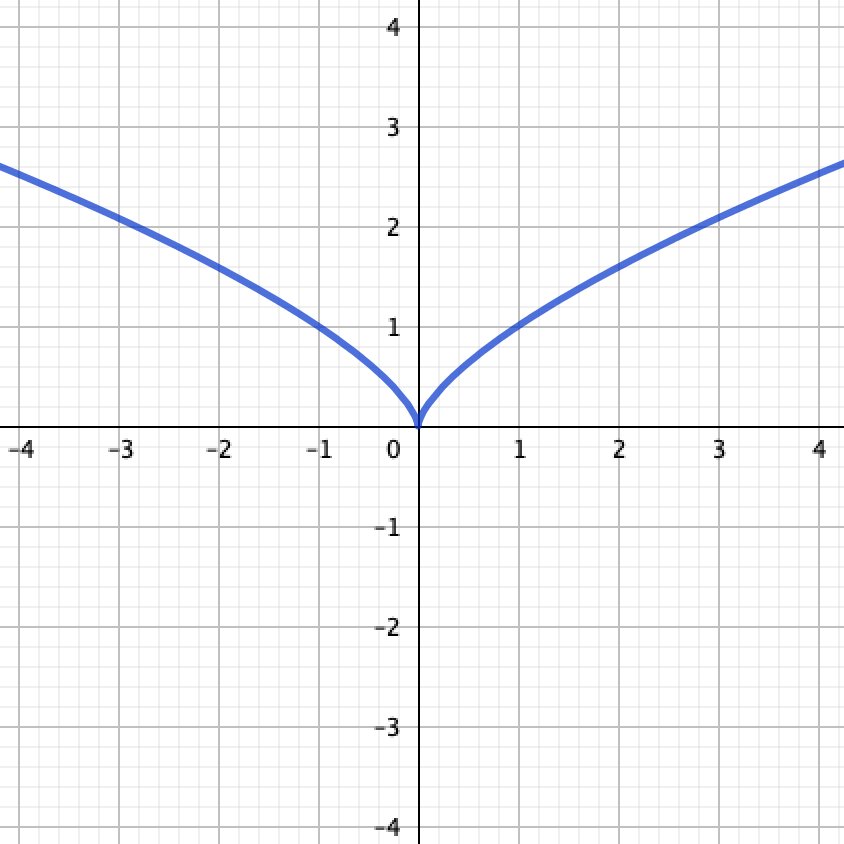
\includegraphics[scale=.5]{curve1}
\end{center}

Note the corner at $(0,0)$; we will see later that this has something to do with our unexpected derivation in the example above.
\end{ex}



\begin{ex} This business about maps of varieties going the wrong way is a bit disorienting. Let's try a couple of examples of this.
\begin{itemize}
\item Given a (radical) ideal $I \subset S=\C[x_1,\dots,x_n]$, the quotient map $S\to S/I$ is given by sending $x_i\mapsto x_i$, so the corresponding map of varieties $V(I)\to \C^n$ is just the inclusion map.
\item Consider $\C[x,y]/(x^2-y^3) \cong \C[t^2,t^3]$ (via $x\mapsto t^3, y\mapsto t^2$) and take the inclusion of rings $\C[t^2,t^3] \subseteq \C[t]$. Under the composition $x\mapsto t^3, y\mapsto t^2$ in $\C[t]$, and corresponding map of varieties goes from $\C\mapsto V(x^2-y^3)$ and sends $b\mapsto(b^3,b^2)$.
\end{itemize}
\end{ex}

One important thing that is \emph{not} included in this correspondence is the usual \emph{Euclidean}\index{Euclidean} topology on $\C^n$ or a subset $X\subseteq \C^n$ with an open basis given by $B_\varepsilon(a) = \{ x \ | \ |x-a|<\varepsilon\}$ with the usual norm $|\cdot |$. We have the \emph{Zariski} topology\index{Zariski} in which the closed sets are subvarieties, but this has no knowledge of what things are close in the Euclidean sense. 

The magic making this all work out so nicely is the Nullstellensatz, which guarantees that maximal ideals of $\C[X]$ all correspond to points of $X$. In general, we just take the (instead of maximal) prime ideals to be our points and work from there.




\begin{center}
\begin{tabular}{c|c}
algebra & ``geometry'' \\ \hline \hline
ring & prime spectrum \\ \hline
 $R$ & $\Spec(R)=\{\fp \ | \ \fp\subset R \ \text{prime ideal}\}$ \\ \hline
prime ideal & point \\ \hline
maximal ideal & closed point \\ \hline
ring homomorphism $R\to S$  & continuous map $Y\to X$ \\
$\phi$ & $\fq \mapsto \phi^{-1}(\fq)$
\end{tabular}
\end{center}

Whereas the correspondence between varieties and reduced f.g. $\C$-algebras was bijective above, the correspondence between rings and their spectra as topological spaces is far from: in particular, every field $K$ has $\Spec(K)$ a singleton. 


\newpage

\sssec{Tangent spaces of varieties}

Let's get to the bottom of this corner business while we're at it. Let's define the \emph{tangent space} of an affine variety $X$ at a point $a$, $T_{a}(X)$. For starters, the tangent space of affine space $\C^n$ at a point $a$ will be the vector space $\C^n$, thought of as centered at $a$. 

\begin{center}
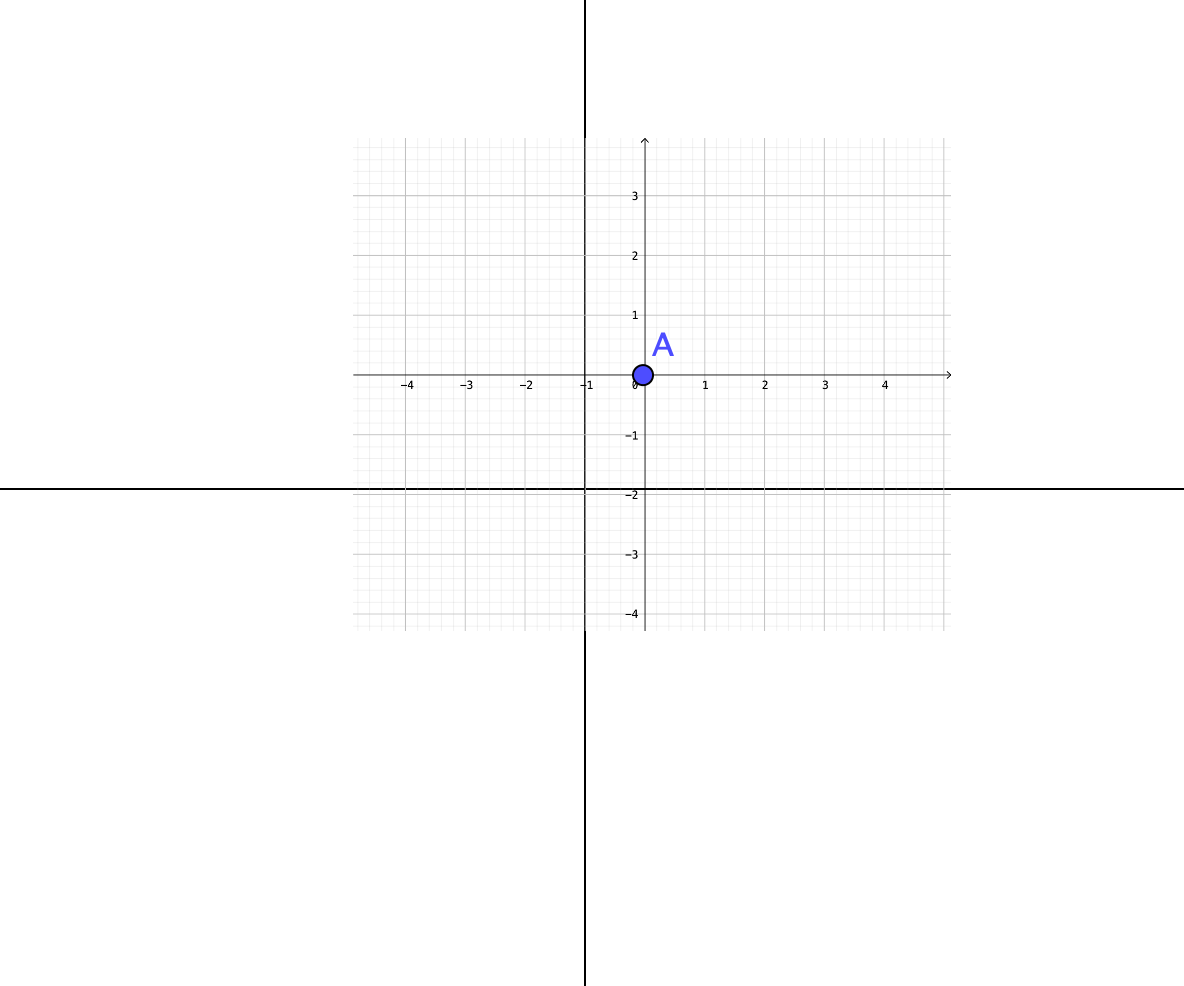
\includegraphics[scale=.4]{tang1}
\end{center}

We can recenter our coordinates there as $\widetilde{x_j}:=x_j-a_j$. Now, given a variety $X=V(f_1,\dots,f_m)$, for each $f_i$ we look at its \emph{linear part}\index{linear part} near $a$: we can take its Taylor expansion at $a$
\[ f_i = f_i(a) + \sum_j \frac{d}{dx_j}|_{x=a}(f_i) (x_j-a_j) + \mathrm{higher \ order \ terms} \ . \]
Since $a\in X$, $f_i(a)=0$, and we have
\[ f_i = \sum_j \frac{d}{dx_j}|_{x=a}(f_i) \widetilde{x_j} + \mathrm{higher\  order\  terms} \ ,\]
so the linear part of $f$ is given by the linear functional $\nabla(f_i)|_{x=a}\cdot \widetilde{x}$. Then we take $T_{a}(X)$ to be the linear subspace of $T_a(\C^n)$ cut out by the linear equations $\nabla(f_1)|_{x=a} v= \cdots = \nabla(f_m)|_{x=a} v = 0$. In particular, $T_a(\C^n)$ is the kernel of the \emph{Jacobian matrix}\index{Jacobian matrix}
\[ J(f_1,\dots,f_m)|_{x=a} = \begin{bmatrix} \frac{d}{dx_1}|_{x=a} (f_1)& \cdots & \frac{d}{dx_n}|_{x=a} (f_1) \\ 
\vdots & \ddots & \vdots \\
\frac{d}{dx_1}|_{x=a} (f_m)& \cdots & \frac{d}{dx_n}|_{x=a} (f_m) \end{bmatrix},\]
whose rows are the gradient vectors.

\Feb{6}
\begin{ex}
Take the parabola $X=V(y - (x-1)^2 -2)$. To compute the tangent space at $a=(1,2)$, take the gradient at $(1,2)$, which is $\begin{bmatrix} -2(x-1) \\ 0\end{bmatrix} |_{(1,2)} =\begin{bmatrix} 0 \\ 1 \end{bmatrix}$, so the defining equation is $\widetilde{y}=0$.
\end{ex}

\begin{center}
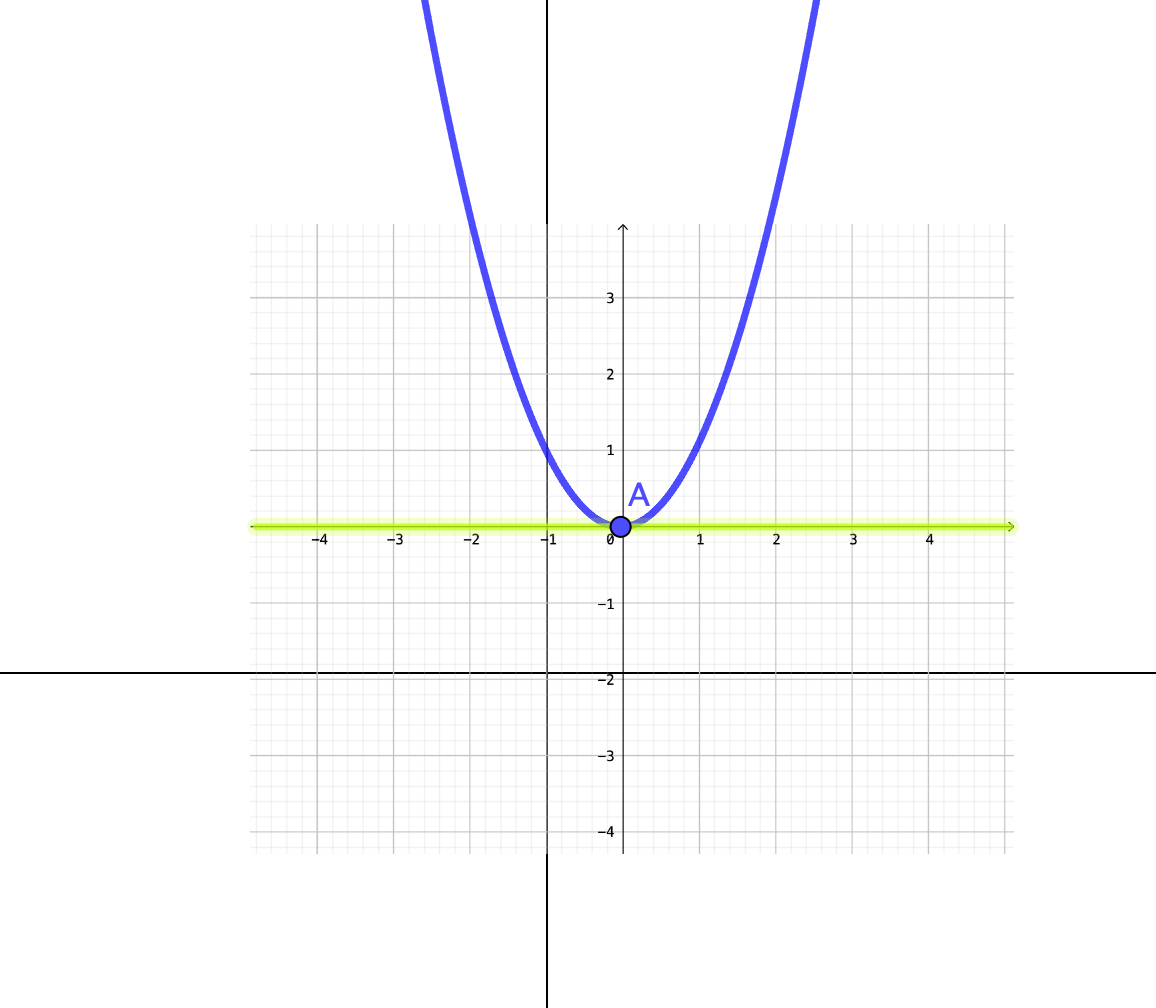
\includegraphics[scale=.4]{tang2}
\end{center}

\begin{ex}
Take the curve $X=V(y^2 - x^3)$. To compute the tangent space at $a=(0,0)$, take the gradient at $(0,0)$, which is $\begin{bmatrix} -3x^2 \\ 2y \end{bmatrix} |_{(0,0)} =\begin{bmatrix} 0 \\ 0  \end{bmatrix}$, so the defining equation is the zero equation. Thus, the tangent space is all of $T_{a}(\C^2)$.
\end{ex}

\begin{center}
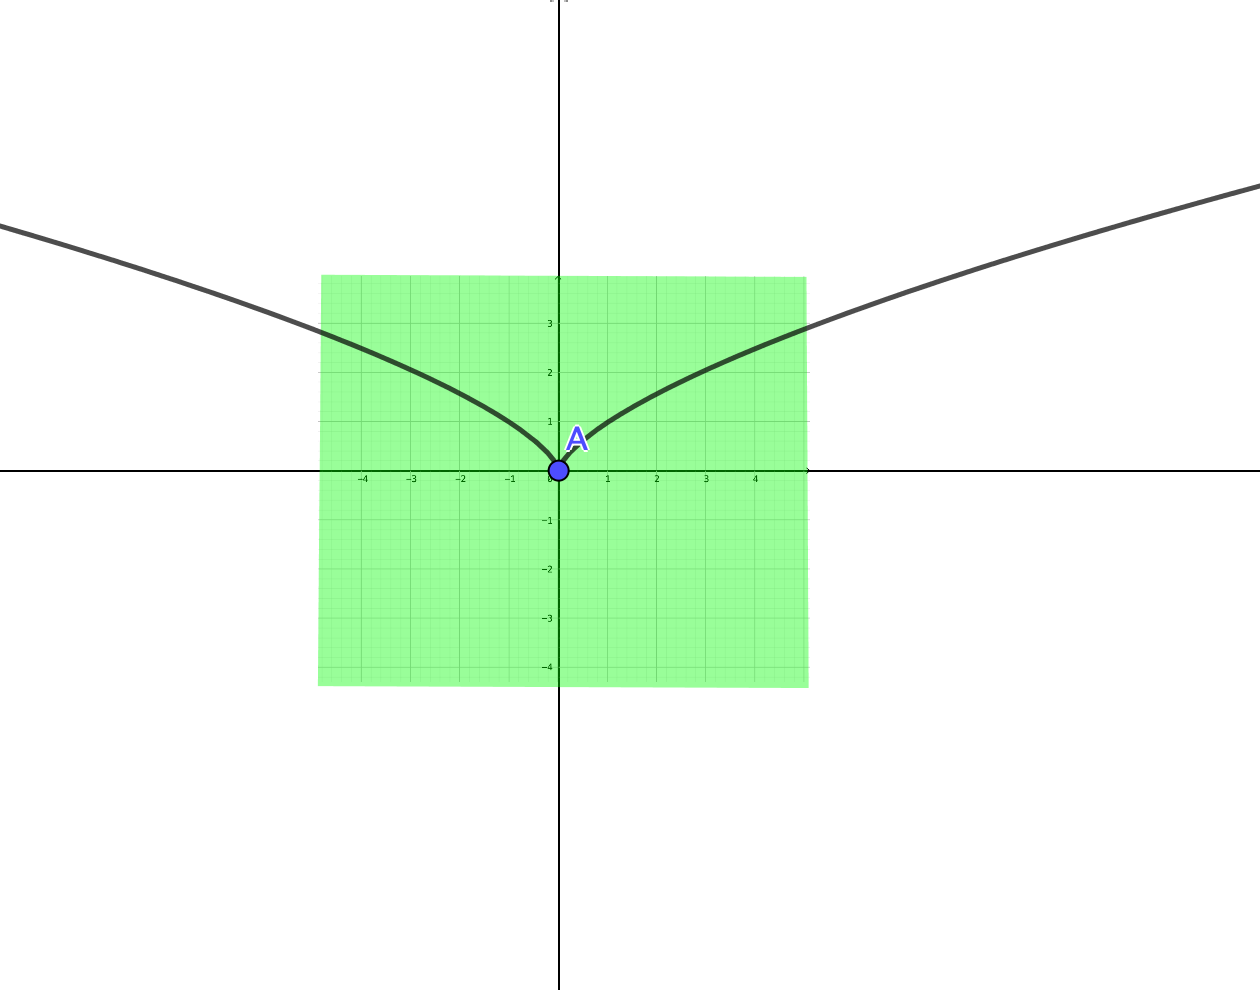
\includegraphics[scale=.4]{tang3}
\end{center}

We want to understand this tangent space in terms of the algebra of the coordinate ring. Here's how.

\begin{prop}
Let $X = V(I)$ be a complex affine variety (with $I$ reduced) and $a\in X$. Let $R=\C[x_1,\dots,x_n]/I$ be the coordinate ring of $X$ and $\fm$ the corresponding maximal ideal. Then there is a $\C$-vector space isomorphism $(\fm/\fm^2)^*\cong T_a(X)$, where $(-)^*$ denotes $\C$-vector space dual.
\end{prop}
\begin{proof} Let $S=\C[x_1,\dots,x_n]$ and $\fn$ be the preimage of $\fm$. Set $\widetilde{x_j} = x_j-a_j$; these are the generators of $\fn$. 
Then  the images of the $\widetilde{x_j}$ form a vector space for $\fn/\fn^2$; we have essentially defined $T_a(\C^n)$ as the $\C$-vector space with coordinates $\widetilde{x_j}$; i.e., the dual space to $\fn/\fn^2$. So $T_a(\C^n)^*\cong \fn/\fn^2$. We will think of $T_a(\C^n)^*= \fn/\fn^2$ each as $1\times n$ row vectors corresponding to the basis $\widetilde{x_j}$ and $T_a(\C^n)$ as $n \times 1$ column vectors.

For an element $f\in \fn$, we can write $f=\nabla(f)|_{x=a}  \widetilde{x}$ in $\fn / \fn^2$, so $\nabla(f)|_{x=a}$ is its row vector.

Then $T_a(X)^*$ corresponds to quotient of the linear functionals on $T_a(\C^n)\to \C$ modulo the ones that vanish on $T_a(X)$. But since $T_a(X)$ is just the set of vectors $v$ such that $\nabla(f_i)|_{x=a} v=0$ for all $i$, a linear functional in $T_a(\C^n)^*$ vanishes on $T_a(X)$ if and only if it is in the (row) span of $\nabla(f_i)|_{x=a}$. Thus, we have \[T_a(X)^* \cong \frac{\fn/\fn^2}{((f_1,\dots,f_m)+\fn^2)/\fn^2} \cong \frac{\fn}{\fn^2+I}.\] Finally, by some basic isomorphism theorems, we can identify $\fm/\fm^2 \cong \fn / (\fn^2+I)$: namely,
\[ \frac{\fm}{\fm^2} \cong \frac{\fn/I}{(\fn^2 + I)/I} \cong \frac{\fn}{\fn^2+I}.\qedhere\]
\end{proof}


\begin{cor} Let $R=\C[X]$ be the coordinate ring of an affine variety and $a\in X$ with associated maximal ideal $\fm$. Then there is an isomorphism $\Der_{R|\C}(R/\fm) \cong T_a(X)$.
\end{cor}

This description of the tangent space of a variety like so is useful; in fact, in many situations, one defines the tangent space to an object by using derivations! Clearly this has some advantages as it naturally arises from $X$ rather than thinking about $X$ inside of $\C^n$ cut out by some equations.



We say that an irreducible affine variety $X$ is \emph{nonsingular} at $a$ if $\dim_\C T_a(X) = \dim X$, and \emph{singular}\index{singular}\index{nonsingular} otherwise (in which case ``$>$'' happens).

\Feb{9}

From the geometric definition of tangent space, we have the following.

\begin{thm}[Jacobian criterion for varieties] Let $X\subseteq \C^n$ be an irreducible affine variety of dimension $d=n-h$. Then
\[ \{a\in X \ | \ X \ \text{is singular at} \ a\} \]
is equal to the vanishing locus of the $h\times h$-minors of $J(f_1,\dots,f_m)$ in $X$.
\end{thm}
\begin{proof}
We have that $T_a(X)=\ker(J(f_1,\dots,f_m)|_{x=a})$, so $\dim(T_a(X)) = n - \mathrm{rank}(J(f_1,\dots,f_m)|_{x=a})$, and so $X$ is singular at $a$ if and only if the rank of $J(f_1,\dots,f_m)|_{x=a}$ is less than $h$. This is equivalent to the all of the $h\times h$ minors of the matrix $J(f_1,\dots,f_m)|_{x=a}$ vanishing. This happens at a point $a$ if and only if each $h\times h$ minor of $J(f_1,\dots,f_m)$ evaluated at $a$ is zero; i.e., $a\in X$ is in the vanishing locus of each $h\times h$ minor.
\end{proof}

\begin{ex} Consider $X=V(x^3-y^2,z-xy)$. The Jacobian matrix is
\[ \begin{bmatrix} 3x^2 & -2y & 0 \\ -y & -x & 1 \end{bmatrix}.\]
Since $X$ has dimension $1$ in $3$ space, we consider the $2\times 2$-minors
\[ -3x^3 - 2y^2, 3x^2, -2y\]
so $x=0, y=0$, and using $z=xy$, $z=0$, and this is the unique singular point on the curve.
\end{ex}


Motivated by the geometric case, for a local ring $(R,\fm,k)$ we define $\fm/\fm^2$ to be the \emph{cotangent space}\index{cotangent space} and $\Hom_k(\fm/\fm^2,k)$ to be the \emph{tangent space}\index{tangent space} of $R$. We recall that a local ring $(R,\fm,k)$ is \emph{regular}\index{regular ring} $\dim(R) = \dim_k(\fm/\fm^2)$.

\begin{ex}
If $R=\C[x_1,\dots,x_n]/I$ is a reduced finitely generated $\C$-algebra, and $\fm$ is a maximal ideal, then $R_{\fm}$ is regular if and only if the variety $X=V(I)$ is nonsingular at $a=V(\fm)$. 
\end{ex}

\begin{ex}
Let $R=\Z_{(2)}$. This is a local ring with maximal ideal $(2)$. The dimension of $R$ is the height of $(2)$ in $\Z$, which is one, and the maximal ideal is generated by one element, so $R$ is regular.
\end{ex}

\begin{ex}
Let $R=\Z[\sqrt{5}]_{(2,1+\sqrt{5})}$. Note that $2,1+\sqrt{5}$ generates a maximal ideal in $\Z[\sqrt{5}]$. The ring $\Z[\sqrt{5}]$ has dimension one, since it is integral over $\Z$, and we see that $R$ has dimension one as well. One can check that the maximal ideal $(2,1+\sqrt{5})$ cannot be generated by one element; equivalently that these elements are $\Z/2\Z$-linearly independent modulo the square of this ideal. Thus, $R$ is not regular.
\end{ex}




\ssec{Localization}
 We include one more property of derivations.
 
 \begin{prop} Let $R$ be an $A$-algebra. Let $W \subseteq R$ be a multiplicative set and $V=W\cap A$. For any $W^{-1}R$ module $M$, any $A$-linear derivation $\partial:R\to M$ extends uniquely to an $A$-linear derivation $W^{-1}R \to M$ given by the rule
 \[\widetilde{\partial}\left(\frac{r}{w}\right) = \frac{w \partial(r) - r\partial(w)}{w^2},\]
 and this extension is $V^{-1}A$-linear. Conversely, any $A$-linear derivation from $W^{-1}R \to M$ is of this form.
 
 That is, there are isomorphisms
 \[ \Der_{R|A}(M) \to  \Der_{W^{-1}R|A}(M) \to  \Der_{W^{-1}R|V^{-1}A}(M).\]
 \end{prop}
 \begin{proof}
 We omit the verification that the rule for the map $W^{-1}R \to M$ is well-defined, that this is $V^{-1}A$-linear, and satisfies the product rule. 
 
 If $\alpha:W^{-1}R \to M$ is an $A$-linear derivation, by restriction through the localization map, we get a derivation $\partial:R\to M$ with $\widetilde{\partial} \circ i = \partial$. We claim that $\alpha=\widetilde{\partial}$. Indeed, \[ \partial(r) = \alpha(r) = \alpha(\frac{r}{w} w) = w \alpha(\frac{r}{w}) + \frac{r}{w} \alpha(w) =  w \alpha(\frac{r}{w}) + \frac{r}{w} \partial(w), \]
 so \[\alpha (\frac{r}{w}) = \frac{ \partial(r)-\frac{r}{w} \partial(w) }{w} = \widetilde{\partial}(\frac{r}{w}).\]
 \end{proof}


\Feb{14}

\ssec{Left-exact sequences}

We now encode many of the key properties of derivations in some left-exact sequences. Recall that a sequence of maps of $R$-modules is  a \emph{left exact sequence}\index{left exact sequence} is an exact sequence of $R$-module maps of the form
\[ 0\to L \xra{\alpha} M \xra{\beta} N.\]
That is, $\alpha$ and $\beta$ are $R$-module homomorphisms such that
with $\alpha$  is injective and $\ker(\beta)=\im(\alpha)$.

\begin{prop} Let $R$ be an $A$-algebra and
\[ 0\to L \xra{\alpha} M \xra{\beta} N\]
be a left exact sequence of $R$-modules. Then
\[ 0\to \Der_{R|A}(L) \xra{\alpha_*} \Der_{R|A}(M) \xra{\beta_*} \Der_{R|A}(N)\]
is a left exact sequence, where $\alpha_*(\partial) = \alpha\circ \partial$ and likewise with $\beta_*$.
\end{prop}
\begin{proof} First we observe that $\alpha_*$ is $R$-linear, since $\alpha_*(\partial+\partial') = \alpha_*\partial + \alpha_*\partial'$ and $\alpha_*(r\partial) = r\alpha_*\partial$. 

Since $\alpha$ is injective, if $\partial\neq 0$, then $\alpha_*\partial\neq 0$. If $\beta_*(\partial)=0$, then $\beta \partial (r)=0$ for all $r\in R$, so $\partial(r)\in \ker(\beta)=\im(\alpha)$ for all $r\in R$, and since $\alpha$ is injective, there is an $R$-linear map $\alpha^{-1}:\im(\alpha) \to L$; then $\partial = \alpha_*(\alpha^{-1} \circ \partial) \in \im(\alpha_*)$.
\end{proof}

\begin{prop} Let $A\to R \xra{\phi} S$ be ring homomorphisms, and $M$ be an $S$-module. Then there is a left exact sequence
\[ 0 \to \Der_{S|R}(M) \xra{\inc} \Der_{S|A}(M) \xra{\phi^*} \Der_{R|A}(M)\]
where $\inc$ is the inclusion map and $\phi^*$ is precomposition with $\phi$.
\end{prop}
\begin{proof}
We start by noting that $\Der_{S|R}(M)$ naturally includes in $\Der_{S|A}(M)$, since any $R$-linear map is automatically linear over the image of $A$. 

If $\partial = \inc(\theta)$, then $\phi^*(\partial) = \partial \circ\phi$ is an $R$-linear derivation on $R$, which must be zero. Conversely, if $\phi^*(\partial) =  \partial \circ\phi$ is zero, then $\phi(R)$ is in the kernel of $\partial$, so $\partial$ is $R$-linear, and hence i the image of $\inc$.
\end{proof}

\begin{prop} Let $A\to R  \xra{\pi} R/I$ be ring homomorphisms, and $M$ be an $R/I$-module. Then there is a left exact sequence
\[ 0 \to \Der_{R/I|A}(M) \xra{\pi^*} \Der_{R|A}(M) \xra{\res} \Hom_R(I/I^2,M). \]
\end{prop}
\begin{proof}
First, we have $\pi^*$ is injective, since if $\partial([r])=0$, then $\pi^*(\partial)(r) = \partial \pi(r) = \partial([r])\neq 0$. 

If $\partial=\pi^*(\theta)$, then $\res( \partial) ([a]) =\theta \circ \pi([a]) = \theta (0)$ for $[a]\in I/I^2$, so $\res\circ\pi^*=0$. Conversely, if $\res(\partial)=0$, then $\partial(a)=0$ for all $a\in I$, so $\partial$ yields a well-defined derivation from $R/I\to M$; i.e., is in the image of~$\pi^*$.
\end{proof}

\begin{prop} Let $A\to R  \xra{\pi} R/I$ be ring homomorphisms, and suppose that there is an $A$-algebra homomorphism $\tau:R/I \to R/I^2$ such that $\tau\pi: R\to R/I^2$ is just the quotient map. Then the sequence
\[ 0 \to \Der_{R/I|A}(M) \xra{\pi^*} \Der_{R|A}(M) \xra{\res} \Hom_R(I/I^2,M) \to 0 \]
is exact.
\end{prop}
\begin{proof}
Follows from the previous, plus proposition on surjectivity of res.
\end{proof}


\sec{Kahler differentials}

\ssec{Restriction and extension of scalars}

\sssec{Hom}


\begin{defn} Let $L,M,N$ be $R$-modules.
	\begin{itemize}
		\item The \emph{module of homomorphisms}\index{module of homomorphisms}\index{$\Hom_R(M,N)$} from $M$ to $N$ is 
		\[ \Hom_R(M,N) := \{ \phi:M \to N \ | \ \phi\text{ is $R$-linear}\}.\]
		The $R$-module structure is given by the rule $r \cdot \phi$ is the homomorphism $m \mapsto r \phi(m) = \phi(rm)$.
		\item If $\alpha: M\to N$ is a module homomorphism, we define a map $\Hom_R(L,\alpha)$ or $\alpha_*$\index{$\Hom_R(L,\alpha)$}\index{$\alpha_*$} from $\Hom_R(L,M)\to \Hom_R(L,N)$ by the rule
		\[ \alpha_*{(\phi)} =  \alpha \circ \phi ;\]
		i.e.,
		\[ \alpha_* : \qquad (\ L\xrightarrow{\phi} M \ ) \ \ \mapsto \ \ (\ L \xrightarrow{\alpha }M\xrightarrow{\phi} N \ ).   \]
			\item If $\alpha: M\to N$ is a module homomorphism, we define a map $\Hom_R(\alpha,L)$ or $\alpha^*$\index{$\Hom_R(\alpha,L)$}\index{$\alpha^*$} from $\Hom_R(N,L)\to \Hom_R(M,L)$ by the rule
		\[ \alpha^*{(\phi)} = \phi \circ \alpha;\]
		i.e.,
		\[ \alpha^* : \qquad (\ N\xrightarrow{\phi} L \ ) \ \ \mapsto \ \ (\ M \xrightarrow{\alpha }N\xrightarrow{\phi} L \ ).   \]
	\end{itemize}
\end{defn}

Thus, given a fixed $R$-module $L$, $F(-):=\Hom_R(L,-)$ is a rule that assigns to any $R$-module $M$ another $R$-module $F(M)$, and to any homomorphism $M \xrightarrow{\phi} N$ a homomorphism $F(M) \xrightarrow{F(\phi)} F(N)$. This plus the fact that $F$ takes the identity map to the identity map and compositions to compositions makes $F$ a \emph{covariant functor}\index{covariant functor} from $R$-modules to $R$-modules.

Similarly, given a fixed $R$-module $L$, $G(-):= \Hom_R(-,L)$ is rule that assigns to any $R$-module $M$ another $R$-module $G(M)$, and to any homomorphism $G(M) \xrightarrow{\phi} G(N)$ a homomorphism $G(N) \xrightarrow{G(\phi)} G(M)$. This plus the fact that $F$ takes the identity map to the identity map and compositions to compositions makes $G$ a \emph{contravariant functor}\index{contravariant functor} from $R$-modules to $R$-modules. The covariant vs.~contravariant bit refers to whether the directions of maps have changed.

Given maps $L \xrightarrow{\alpha} L'$ and $M \xrightarrow{\beta} M'$, we likewise get a map $\Hom_R(L',M) \xrightarrow{\Hom_R(\alpha,\beta)} \Hom_R(L,M')$, by combining the constructions above.

\begin{ex}
$\Hom_R(R,M)\cong M$ by $\phi\mapsto \phi(1)$, and under this isomorphism, $M \xrightarrow{\alpha} N$ corresponds to $1 \mapsto m \rightsquigarrow 1 \mapsto \alpha(m)$ under this isomorphism.

If $I$ is an ideal, $\Hom_R(R/I,M)\cong \ann_M(I)$ by the same map: the image of $1$ in $R/I$ must map to something killed by $I$, and there is a unique $R$-linear map that does this. The same recipe for maps as above holds. Thus, we can identify $\Hom_R(R/I,-)$ with the functor that sends modules $M$ to $\ann_M(I)$, and sends maps to their restrictions to these submodules.
\end{ex}

We recall that a sequence of maps of $R$-modules is \emph{split-exact} if it is of the form
\[ 0 \to L \xra{\alpha} M \xra{\beta} N \to 0\]
with $\alpha$ injective, $\beta$ surjective, $\ker(\beta)=\im(\alpha)$ and $\alpha$ has a left inverse (i.e., there is a map $\rho$ such that $\rho \alpha$ is the identity on $L$). It is equivalent if we replace the last condition with $\beta$ has a right inverse (i.e., there is a map $\iota$ such that $\beta \iota$ is the identity on $N$.

\begin{thm}
	\begin{enumerate}
		 \item	A sequence of maps \[ 0 \to L \xrightarrow{\alpha} M \xrightarrow{\beta} N\]
		is exact if and only if, for all $R$-modules $X$, the sequence
		\[ 0 \to \Hom_R(X,L) \xrightarrow{\alpha_*} \Hom_R(X,M) \xrightarrow{\beta_*} \Hom_R(X,N)  \]
		is exact.
		\item A sequence of maps \[ 0 \to L \xra{\alpha} M \xra{\beta} N \to 0\] is split-exact if and only if, for all $R$-modules $X$, the sequence
		\[ 0 \to \Hom_R(X,L) \xrightarrow{\alpha_*} \Hom_R(X,M) \xrightarrow{\beta_*} \Hom_R(X,N) \to 0 \]
		is exact.

\item	A sequence of maps \[ L \xrightarrow{\alpha} M \xrightarrow{\beta} N \to 0 \]
is right-exact if and only if, for all $R$-modules $X$, the sequence
\[ 0 \to \Hom_R(N,X) \xrightarrow{\beta^*} \Hom_R(M,X) \xrightarrow{\alpha^*} \Hom_R(L,X)  \]
is left-exact.
\item A sequence of maps \[ 0 \to L \xra{\alpha} M \xra{\beta} N \to 0\] is split-exact if and only if, for all $R$-modules $X$, the sequence
\[ 0 \to \Hom_R(N,X) \xrightarrow{\beta^*} \Hom_R(M,X) \xrightarrow{\alpha^*} \Hom_R(L,X) \to 0 \]
is exact.
\end{enumerate}
\end{thm}
\begin{proof}
\begin{enumerate}
\item
 Let $0 \to L \xrightarrow{\alpha} M \xrightarrow{\beta} N$ be exact, and $X$ be an $R$-module. 
 \begin{itemize}
 \item $\alpha_*$ is injective: if $X \xrightarrow{\phi} L$ is nonzero, $X \xrightarrow{\phi} L \xrightarrow{\alpha} M$ is as well, since a nonzero element in the image of $\phi$ goes to something nonzero in the composition.
\item $\ker(\beta_*)=\im(\alpha_*)$: $X \xrightarrow{\phi} M \xrightarrow{\beta} N$ is zero if and only if $\im(\phi) \subseteq \ker(\beta) = \im(\alpha)$, which happens if and only if $\phi$ factors through $L$; i.e., $\phi\in \im(\alpha_*)$.
\end{itemize}

  The other direction of the first part follows from the example above; we can use $X=R$.

\item Let $0 \to L \xrightarrow{\alpha} M \xrightarrow{\beta} N \to 0$ be split-exact, and $X$ be an $R$-module. In particular, $0 \to L \xrightarrow{\alpha} M \xrightarrow{\beta} N$ is a left exact sequence, so 
\[ 0 \to \Hom_R(X,L) \xrightarrow{\alpha_*} \Hom_R(X,M) \xrightarrow{\beta_*} \Hom_R(X,N)  \]
		is exact. We just need to see that $\Hom_R(X,M) \xrightarrow{\beta_*} \Hom_R(X,N) $ is surjective. Let $\iota$ be such that $\beta\iota$ is the identity on $N$. Then $\beta_*\iota_*$ is the identity on $\Hom_R(X,M)$, so $\beta_*$ must be surjective.
		
		For the converse, take $X=N$. Then the identity map in $\Hom_R(N,N)$ is in the image of $\beta_*$, so there is a map $\rho\in \Hom_R(M,N)$ such that $\beta \rho =\beta_*(\rho)$ is the identity on $N$, as required.
 
\item  Let $L \xrightarrow{\alpha} M \xrightarrow{\beta} N \to 0$ be a right-exact sequence, and $X$ be an $R$-module.
  \begin{itemize}
\item   $\beta^*$ is injective: if $N \xrightarrow{\phi} X$ is nonzero, pick $n\in N$ not in the kernel, and $m\in M$ that maps to $n$. Then, the image of $m$ under $ M \xrightarrow{\beta} N \xrightarrow{\phi} X$ is nonzero.
 \item $\ker(\alpha^*)=\im(\beta_*)$: $ L \xrightarrow{\alpha} M \xrightarrow{\phi} X$ is zero if and only if $\im(\alpha)\subseteq \ker(\phi)$, which happens if and only if $\phi$ descends to a map of the form $N \cong M/\im(\alpha) \to X$; i.e., $\phi \in \im(\alpha^*)$.
\end{itemize}
 Let $L \xrightarrow{\alpha} M \xrightarrow{\beta} N \to 0$ be a sequence of maps, and suppose that it is exact after applying $\Hom_R(-,X)$ for all $X$.
  
   \begin{itemize}\item $\beta$ is surjective: if not, let $X=N/\im(\beta)$. There is a nonzero projection map $N \xrightarrow{\phi} X$, but $M \xrightarrow{\beta} N \xrightarrow{\phi} X$ is zero, contradicting injectivity of $\beta^*$.
\item  $\ker(\beta)\supseteq \im(\alpha)$: Take $X=N$, and $N\xrightarrow{\mathrm{id}} X$. Since $\ker(\alpha^*)\supseteq \im(\beta^*)$, $L \xrightarrow{\alpha} M \xrightarrow{\beta} N\xrightarrow{\mathrm{id}} X = L \xrightarrow{\alpha} M \xrightarrow{\beta} N$ is zero.
 \item $\ker(\beta)\subseteq \im(\alpha)$: Take $X=M/\im(\alpha)$, and $M \xrightarrow{\phi} X$ the projection map. Since $L \xrightarrow{\alpha} M \xrightarrow{\phi} X$ is zero, $\phi$ is in the image of $\beta^*$, so it factors through $\beta$. This is equivalent to the stated containment.
 \end{itemize}
 
 \item Similar to (2). \qedhere
 
 \end{enumerate}
 
\end{proof}

In short, $\Hom_R(X,-)$ is kernel-preserving, and $\Hom_R(-,X)$ turns cokernels into kernels.

Given a ring homomorphism $\phi:R\to S$, we can use $\phi$ to turn $S$-modules and $S$-algebras into $R$-modules and $R$-algebras with \emph{restriction of scalars} and vice versa with \emph{extension of scalars}.

\sssec{Restriction of scalars}

Given $\phi:R\to S$ and an $S$-module $N$, we get an $R$-module $\phi_*(N)$\index{$\phi_*$} by \emph{restriction of scalars}\index{restriction of scalars} by keeping the same set and same addition, so $\phi_*(N)=N$ as additive groups, and the $R$-module action $r\cdot  n := \phi(r) \cdot n$, where the left-hand side is the action in $\phi_*(N)$ and the right hand side is the original $S$-action. When $\phi: R\to S$ is just an inclusion map $R\subseteq S$, this restriction of scalars is literally just restricting which scalars we consider in the module action. 

For example, consider $R=\C \subseteq S=\C[x]$ and $N=\C[x]/(x^3)$. $N$ is a cyclic $S$-module killed by some stuff, but we can also ``forget about the action of $x$'' and consider $N$ as a $\C$-vectorspace; as such it is just a free $3$-generated $R$-module.

Given a homomorphism of $S$-modules $\alpha:N \to N'$, we can call $\phi_*(\alpha)$ the same map from $\phi_*(N)\to \phi*(N)$, which is a homomorphism of $R$-modules.

We can think of this restriction of scalars $\phi_*$ as the ``demotion''\index{demotion} functor, when demotes modules from a ``bigger'' (target of $\phi$) ring to a ``smaller'' (source of $\phi$) ring.

In the same way, we can demote $S$-algebras to $R$-algebras: if $T$ is an $S$-algebra with structure map $\psi:S\to T$ take $\phi_*(T)$ to be the same ring $T$ with structure map $\psi\circ \phi:R\to T$.

To promote a module or an algebra, we have to do something a bit more interesting. For example, consider $R= \C \subseteq S=\C[x]$ and $M=\C^3$, a free $R$-module of rank $3$. There is no ``obvious'' or ``natural'' $R$-module structure on $M$, so we'll end up changing our underlying set. The ``right'' way of going about this is by using tensor products, but we'll take a barehanded approach using presentations, and everyone is encouraged to reconcile the two approaches now if they know tensors and, if not, later when they do.

\sssec{Presentations of modules}

Let $M$ be an $R$-module.

Given a generating set $\{m_\lambda\}_{\lambda\in \Lambda}$ for $M$, there is a surjection from a free module onto $M$:
\[\xymatrix@R=0pc{  \{m_\lambda\}_{\lambda\in \Lambda}  & \rightsquigarrow & R^{\oplus \Lambda} \to M \to 0 \\  \text{generating set} & &  e_\lambda \mapsto m_\lambda \ \ \ }\]
and conversely any such surjection yields a generating set (consisting of the images of the basis vectors).

The kernel of this map is a submodule of $R^{\oplus \Lambda}$ which are the relations on these generators. We can take a subset $\{v_\gamma\}_{\gamma\in \Gamma}$ that generates the module of relations (a set of \emph{defining relations}) and map a free module onto them:
\[\xymatrix@R=0pc@C=.5pc{  \{m_\lambda\}_{\lambda\in \Lambda}  & + & \{v_\gamma\}_{\gamma\in \Gamma} &  \rightsquigarrow & R^{\oplus \Gamma} \longrightarrow R^{\oplus \Lambda} \longrightarrow M \to 0 \\  \text{generating set} & & \text{defining relations} &  & e'_\gamma \mapsto v_\gamma \ \ e_\lambda \mapsto m_\lambda \ \ \ \ }\]
Conversely, any such right exact sequence is a recipe for a set of generators and defining relations on $M$. The map between free modules is given by multiplication by a (possibly infinite) matrix $A$ whose $\gamma$ column consists of the $\lambda$-coordinates of $v_\gamma$; concretely, each column is a relation on the $m_\lambda$'s. When $\Lambda$ and $\Gamma$ are finite, we'll just write something like
\[ R^m \xrightarrow{A} R^n \to M \to 0\]
and $A$ will be an actual $n\times m$ matrix, standing for the map of  multiplication (on the left) by $A$. We will call this (either in the finite or infinite case) a \emph{presentation matrix}\index{presentation matrix} for $M$. 

Given a presentation matrix, we can recover $M$ up to isomorphism as $M\cong R^n/\im(A)$ (i.e., the \emph{cokernel}\index{cokernel} of the map $A$) coming from the first isomorphism theorem, since the map from $R^n\to M$ is surjective with kernel $\im(A)$. The rows of the presentation matrix correspond to generators, and the columns correspond to relations.






\sssec{Extension of scalars for modules}
We're now ready to describe \emph{extension of scalars}\index{extension of scalars}, or \emph{promotion}\index{promotion} of a module along a ring homomorphism. Let $\phi:R\to S$ be a ring homomorphism and $M$ be an $R$-module. We define the extension of scalars of $M$, denoted $\phi^*(M)$ or $S\otimes_R M$\index{$\phi^*(M)$}\index{$S\otimes_R M$} as follows. Take a presentation of $M$:
\[ R^m \xra{A} R^n \to M \to 0;\]
then $\phi^*(M)$ is the $S$-module with the same presentation
\[ S^m \xra{\phi(A)} S^n \to \phi^*(M) \to 0.\]

\Feb{16}

It's not clear that what we did does not depend on the choice of presentation. However, we will show that the $\phi^*(M)$ satisfies an important universal property and use that to show it is well-defined.

First we note that there is an $R$-module homomorphism from $\eta_M: M \to \phi^*(M)$ (or more properly, to $\phi_*\phi^*(M)$). Given $r\in R$ write $m= \sum_i r_i [e_i]$, where the $e_i$'s are the standard basis in $R^n$. For convenience, set $\mathbf{e}$ to be the row vector with entries $e_1,\dots,e_n$ and $\mathbf{r}$ be the column vector of $r_1,\dots, r_n$ so $m= \mathbf{e}\mathbf{r}$. We map $m$ to $\mathbf{e} \phi(\mathbf{r}) = \sum_i \phi(r_i) [e_i]$. If $m$ also equals $\sum_i r'_i [e_i] = \mathbf{e}\mathbf{r'}$, then $\mathbf{e}(\mathbf{r}-\mathbf{r'})= 0$ so $\mathbf{r}-\mathbf{r'} = A\mathbf{v}$ for some $\mathbf{v}$, and hence \[ \mathbf{e} \phi(\mathbf{r}) - \mathbf{e} \phi(\mathbf{r'}) = \mathbf{e} \phi(\mathbf{r}-\mathbf{r'}) = \mathbf{e} \phi(A\mathbf{v}) = \mathbf{e} \phi(A) \mathbf{v},\]
so this is zero in $\phi^*(M)$. It is then clear to see that this is $R$-linear. 

\begin{prop}
Let $\phi:R\to S$ be a ring homomorphism. Let $M$ be an $R$-module, $N$ be an $S$-module, and $\alpha:M \to \phi_*(N)$ be an $R$-module homomorphism. Then there exists a unique $S$-module homomorphism $\beta: \phi_*(M) \to N$ that makes the diagram commute:
\[ \xymatrix{  M \ar[r]^-{\eta_M} \ar[dr]_-{\alpha} & \phi^*(M) \ar@{-->}[d]^-{\beta} \\ & N}.\]
\end{prop}
\begin{proof} We will abuse notation and drop the $\phi$ to identify elements in $R$ with their images in $S$.

Let $\alpha([e_i]) = n_i$ and write $\bs{n}$ for the row vector $[n_1,\dots,n_t]$. We define $\beta( \sum_i s_i [e'_i] ) = \sum_i s_i n_i$, or $\beta(\mathbf{e}\mathbf{s}) = \mathbf{n}\mathbf{s}$ for short. To see that this is well-defined, suppose that $\sum_i s_i [e'_i] = \sum_i s'_i [e'_i]$, and write $\bs{s}$ and $\bs{s'}$ for the column vectors of $s_i$ and $s'_i$. We need to show that $\bs{n}\bs{s}=\bs{n}\bs{s'}$. By construction of $\phi^*(M)$, we have that $\bs{s}-\bs{s'} = A \bs{v}$ for some vector $\bs{v}$ with entries in $S$. Since $\alpha$ is well-defined, we must have that for any columns of $A$, the corresponding combination of basis vectors maps to zero, so the corresponding combination of the $n$'s is zero; i.e., $\bs{n} A=0$. But then $\bs{n} A \bs{v} = \bs{n} (\bs{s}-\bs{s'})$, and this shows the claim. Checking $S$-linearity is straightforward from the construction.
 For uniqueness, $\phi^*(M)$ is generated by $[e_i]$, and $n_i = \alpha([e_i])= \beta \eta_M([e_i])=\beta([e'_i])$, so the generators must go to the same place, and hence there can only be one map.
\end{proof}

In other words, the proposition says that for any $R$-module $M$ and $S$-module $N$, there is an isomorphism 
\[  \Hom_S(\phi^*M,N) \xra{\eta_M^*} \Hom_R(M,\phi_* N).\]

\begin{cor}
 $\phi:R\to S$ be a ring homomorphism, and $M$ be an $R$-module. Fix two presentations for $M$, and let $(\phi_1^*(M),\eta^M_1)$ and $(\phi^*_2(M), \eta^M_2)$ be the two modules and morphisms constructed above for each presentation. Then $\phi^*_1(M)\cong \phi^*_2(M)$ as $S$-modules. Moreover, there is a unique $S$-module isomorphism $\theta$ for which $\eta^M_2 = \theta \circ \eta^M_1$.
\end{cor}
\begin{proof}
It suffices to show that there is an isomorphism that makes $\eta^M_2 = \theta \circ \eta^M_1$, for the uniqueness will follow from the proposition applied with $\alpha=\eta_2$.
Consider the diagram
\[ \xymatrix{ & \phi^*_1(M) \ar@{-->}[d]\\
M \ar[ur]^{\eta_1} \ar[r]^{\eta_2} \ar[dr]_{\eta_1} & \phi^*_2(M)\ar@{-->}[d] \\
& \phi^*_1(M)}\]
The universal property yields unique $S$-module dotted maps making the triangles commute. The double down composition and the identity map on $\phi^*_1(M)$ are two maps that make the big triangle commute. Applying the uniqueness in the proposition with $\alpha=\eta_1$, we get that the composition is the identity. We can switch the roles of $\phi^*_1$ and $\phi^*_2$ to get that the other composition is the identity. Thus, the induced map is an isomorphism.
\end{proof}

\begin{cor}
Let $\phi:R\to S$ be a ring homomorphism. For any $R$-module homomorphism $\alpha:M\to N$, there is a unique $S$-module homomomorphism $\phi^*\alpha:\phi^*M \to \phi^*N$ such that $\phi^*\alpha \circ \eta_M = \eta_N \circ \alpha$.
\end{cor}
\begin{proof} 
Apply the universal property of $(\phi^*M, \eta_M)$ to $\eta_N \circ \alpha$.
\end{proof}

Tracing the proof of the universal property, we see that $\phi^*\alpha$ can be computed as follows: take presentations for $M$ and $N$, and
lift $\alpha$ to a matrix from the free modules over $M$ and $N$; then use the same matrix for $\phi^*\alpha$.

\begin{lem} Under the isomorphisms $\Hom_S(\phi^*M,N) \xra{\eta_M^*} \Hom_R(M,\phi_* N)$, the map $\Hom_S(\phi^*\alpha,N)$ corresponds to $\Hom_R(\alpha,N)$.
That is, for an $R$-module homomorphism $\alpha:L\to M$ and $S$-module $N$, there is a commutative diagram:
\[\xymatrix@C=5em{
 \Hom_S(\phi^* M, N) \ar[r]^{\Hom_S(\phi^*\alpha,N)} \ar[d]^{\eta_M^*}_{\cong} &  \Hom_S(\phi^* L, N) \ar[d]^{\eta_L^*}_{\cong} \\
 \Hom_R(M,N) \ar[r]^{\Hom_R(\alpha,N)} & \Hom_R(L,N)
}\]
\end{lem}
\begin{proof}
First, by construction of $\phi^*\alpha$, we have a commutative diagram:
\[ \xymatrix{
\phi^*M & \ar[l]_{\phi^* \alpha} \phi^* L \\
M \ar[u]_{\eta_M} & L \ar[l]_{\alpha} \ar[u]_{\eta_L}}\]
Then using this commutativity, given an $S$-linear map $\theta:\phi^*M \to N$, we have that
\[(\eta_L^* \circ \Hom(\phi^*\alpha,N)) (\theta) = \theta \circ \phi^*\alpha \circ \eta_L = \theta \circ \alpha \circ \eta_M = (\Hom(\alpha,N) \circ \eta_M^*)(\theta).\qedhere\]
\end{proof}

\begin{prop} Let $\phi:R\to S$ be a ring homomorphism, and 
\[ L \xra{\alpha} M \xra{\beta} N \to 0\]
be a right exact sequence of $R$-modules. Then the sequence of $S$-modules
\[ \phi^*L \xra{\phi^*\alpha} \phi^*M \xra{\phi^*\beta} \phi^*N \to 0\]
is exact.
\end{prop}
\begin{proof}
Let $X$ be an arbitrary $S$-module. Applying Hom into $X$ to the sequence above, we have a sequence:
\[ 0 \to \Hom_S(\phi^*N,X)  \xra{\Hom(\phi^*\beta,X)} \Hom_S(\phi^*M,X) \xra{\Hom(\phi^*\alpha,X)} \Hom_S(\phi^*L,X).\]
We have isomorphisms
\[ \xymatrix@C=5em{ 
0 \ar[r] \ar@{=}[d]  & \Hom_S(\phi^*N,X)  \ar[r]^{\Hom(\phi^*\beta,X)} \ar@{=}[d] & \Hom_S(\phi^*M,X) \ar[r]^{\Hom(\phi^*\alpha,X)} \ar@{=}[d] & \Hom_S(\phi^*L,X) \ar@{=}[d] \\
0 \ar[r] & \Hom_R(N,X) \ar[r]^{\Hom(\beta,X)} & \Hom_R(M,X) \ar[r]^{\Hom(\alpha,X)} & \Hom_R(L,X) }\]
The last row is exact, by left exactness of Hom (part (3) in the forward implication). But then by left exactness of Hom again, since this is true for all $X$, the sequence we consider is exact.
\end{proof}

In general, exact sequences (or left exact sequences) no longer remain exact. We say that a ring homomorphism $\phi:R\to S$ is \emph{flat}\index{flat} if it has the special property that extension of scalars preserves exact sequences.

\begin{prop} Let $R$ be a ring and $W$ be a multiplicative set. Let $\phi:R\to W^{-1}R$ be the localization map. Then $\phi^*(M)\cong W^{-1}M$ for any $R$-module $M$.
\end{prop}
\begin{proof} Let $\eta:M \to W^{-1}M$ be the localization map. We will show that $(W^{-1}M,\eta)$ satisfies the universal property of $\phi^*M$. If $N$ is any $W^{-1}R$-module, and $\alpha:M\to N$ is a homomorphism, define $\beta:W^{-1}M \to N$ by sending $\beta(\frac{m}{w}) = \frac{\alpha(m)}{w}$. The check that this $\beta$ is well-defined and $W^{-1}R$-linear is straightforward; that it is the unique map making the diagram commute follows from the fact that the image of $M$ generates $W^{-1}M$ as a $W^{-1}R$-module.
\end{proof}





\sssec{Presentations of algebras}
We can play a similar game with algebras. Let $S$ be an $R$-algebra, so there is some $\phi:R\to S$. Given a generating set for $S$ as an algebra, we get a surjection from a polynomial ring:
\[\xymatrix@R=0pc{  \{s_\lambda\}_{\lambda\in \Lambda}  & \rightsquigarrow & R[\{x_\lambda\}_{\lambda\in\Lambda}] \to S  \to 0 \\  \text{algebra generating set} & & \ \ \ \ \ \ x_\lambda \mapsto s_\lambda }\]
The kernel is an ideal $I$, for which we can pick generators $(\{f_\gamma\}_{\gamma\in \Gamma})$ and we get
\[\xymatrix@R=0pc@C=.5pc{  \{s_\lambda\}_{\lambda\in \Lambda}  & + & \{f_\gamma\}_{\gamma\in \Gamma} &  \rightsquigarrow & R[\{x_\lambda\}_{\lambda\in\Lambda}]^{\oplus \Gamma}  \longrightarrow R[\{X_\lambda\}_{\lambda\in\Lambda}] \longrightarrow S \to 0 \\  \text{algebra generating set} & & \text{defining relations} &  & \quad \qquad e'_\gamma \mapsto f_\gamma \qquad \qquad e_\lambda \mapsto s_\lambda }\]
Note that we have \emph{polynomial} relations rather than linear relations now, so we can't use a matrix to describe them anymore. 


Given an $R$-algebra $S$ with an algebra presentation $S\cong R[x_1,\dots,x_n]/(f_1,\dots,f_m)$, we can also ask what $S$ looks like as an $R$-module. As a generating set, we can take the monomials $\{x_1^{a_1}\cdots x_n^{a_n} \ | \ a_i\in \N\}$. The relations are generated as an $R[x_1,\dots,x_n]$-module by $f_1,\dots, f_m$; to find an $R$-module generating set of the relations, we can take $\{ x_1^{a_1}\cdots x_n^{a_n} f_j \ | \ a_i\in \N, j=1,\dots,m\}$ and collect the coefficients of the monomials, and this gives a presentation. That is, if $f_j = \sum_a c_{a,j} x^a$ for some tuples $a$, then $\{\sum_a c_{a,j} x^{a+b} \ | \ b\in \N^n, j=1,\dots,m\}$ is a defining set of relations. 

For example, consider $R=\Z[x]/(2x^2-5)$. Let's find a $\Z$-module presentation of this ring. As a generating set, we have $1,x,x^2,x^3,\dots$; the relations are given by $2x^2-5, 2x^3 -5x, 2x^4-5x^2, \dots$; the presentation matrix is
\[ \begin{bmatrix} 
-5 & 0 & \cdots & & \\
0 & -5 & 0 & \cdots & \\
2 & 0 & -5 & 0 & \cdots \\
0 & 2 & 0 & -5 & \ddots \\
& \ddots & \ddots & \ddots & \ddots \end{bmatrix}\]



\sssec{Base change for algebras}


Let's promote some algebras too. We'll follow the same recipe: take a presentation (as an algebra) and upgrade the base ring. That is, let $\phi:R\to S$ be a ring homomorphism and $T$ be an $R$-algebra. We define the \emph{extension of scalars}\index{extension of scalars} or \emph{base change}\index{base change} of $T$ as follows. Write
\[ R[X_1,\dots,X_n]^{m} \xra{[f_1,\dots,f_m]} R[X_1,\dots,X_n] \to T \to 0;\]
then $\phi^*(T)$ is the $S$-algebra with presentation
\[ S[X_1,\dots,X_n]^{m} \xra{[\phi(f_1),\dots,\phi(f_m)]} S[X_1,\dots,X_n] \to \phi^*(T) \to 0.\]

Note that we are using the same notation as module extension of scalars, though it is not immediately clear these should be related. For starters, in analogy with the module extension of scalars, one has:

\begin{prop} For a ring homomorphism $\phi:R\to S$ and an $R$-algebra $T$, the base change $\phi^*T$ 
admits an $R$-algebra homomorphism $\eta_T: T\to \phi^*T$ that satisfies the universal property that for any $S$-algebra $V$ and $R$-algebra homomorphism $\alpha:R\to V$, there is a unique $S$-algebra homomorphism $\beta: \phi^*T\to V$ that makes the diagram commute:
\[  \xymatrix{  T \ar[r]^-{\eta_T} \ar[dr]_-{\alpha} & \phi^*T \ar@{-->}[d]^-{\beta} \\ & V}.\]
Consequently, $\phi^*T$ is well-defined (independent of the choice of presentation) up to isomorphism.
\end{prop}
\begin{proof} Omitted; similar to what we did with modules.
\end{proof}

Another key point is that this base change operation for algebras agrees with that for modules. Namely:

\begin{prop} Let $\phi:R\to S$ be a ring homomorphism and $T$ an $R$-algebra. Then the $S$-algebra $\phi^* T$ obtained by extension of scalars of $R$-algebras along $\phi$, considered as an $S$-module, is isomorphic to the extension of scalars of $T$ considered as an $S$-module.
\end{prop}
\begin{proof}
Take a presentation of $T$ as an $R$-algebra, and take the presentation as an $R$-module obtained from it as discussed above, i.e., with relations $\{\sum_a c_{a,j} x^{a+b} \ | \ b\in \N^n, j=1,\dots,m\}$ for an algebra generating set $f_j=\sum_a c_{a,j} x^a$. If we take algebra extension of scalars of $T$, then we get the same presentation as an $S$-module by this formula.
\end{proof}

\ssec{Kahler differentials}

\begin{defn} Let $R$ be an $A$-algebra. A derivation $d_{R|A}:R\to \Omega_{R|A}$ to some $R$-module $\Omega_{R|A}$ is called a \emph{universal derivation}\index{universal derivation} of $R$ over $A$ if for any $A$-linear derivation $\partial:R\to M$ to any $R$-module $M$, there is a unique $R$-module homomorphism $\alpha:\Omega_{R|A}\to M$ such that $\partial = \alpha\circ d_{R|A}$:
\[  \xymatrix{  R \ar[r]^-{d_{R|A}} \ar[dr]_-{\partial} & \Omega_{R|A} \ar@{-->}[d]^-{\alpha} \\ & M}.\]
We call the target module $\Omega_{R|A}$ a \emph{module of differentials} or module of \emph{Kahler differentials} of $R$ over $A$.
\end{defn}

\begin{thm} Let $R$ be an $A$-algebra. There exists a universal derivation of $R$ over $A$. Given two universal derivations $d_{R|A}:R\to\Omega_{R|A}$ and $d'_{R|A}:R\to \Omega'_{R|A}$ of $R$ over $A$, there is a unique isomorphism $\alpha:\Omega_{R|A} \cong \Omega'_{R|A}$ such that $\alpha d = d'$. In particular, there exists a module of differentials that is unique up to isomorphism.
\end{thm}
\begin{proof}
\textbf{Existence of universal derivation:} Let $F$ be a free module with basis $\{dr \ | \ r\in R\}$, and $d:R\to F$ be function $d(r) = dr$. (Note that this function is not a  homomorphism in any sense, just a function.) Let $J$ be the submodule of $F$ generated by the elements of the form
\begin{itemize}
\item $d(r+s) - dr -ds$, $r,s\in R$,
\item $d(rs) = r ds - s dr$, $r,s\in R$,
\item $d(ar) = a dr$, $a\in A$, $r\in R$,
\end{itemize}
and set $\Omega=F/J$, and by abuse of notation $d$ the map $R\to \Omega$. First, we observe that $d$ is an $A$-linear derivation: the relations in $J$ force each rule to hold.
Now, suppose that $\partial:R\to M$ is a derivation. We need to see that there is exactly one $R$-module homomorphism $\alpha:\Omega\to M$ such that $\alpha\circ d = \partial$.
There is at most one, since $\Omega$ is generated by the elements $dr$ and $\alpha(dr) = \alpha(d(r)) = \partial(r)$, so the images of the generators are determined. To see that the map $\alpha:F\to M$ given on the generators $dr$ as $\alpha(dr) = \partial(r)$ gives a well-defined $R$-module homomorphism $\alpha:\Omega\to M$, we just need to check that $\alpha(J)=0$, or equivalently that $\alpha$ maps each of the generators of $J$ to zero. But $\alpha( d(r+s) - dr - ds ) = \partial(r+s) - \partial(r) - \partial(s) = 0$, and similarly for the other rules since $\partial$ is an $A$-linear derivation. Thus, such a map $\alpha$ exists (and, still, is unique). This shows that $d:R\to \Omega$ is a universal derivation.

\textbf{Uniqueness of universal derivation:} This is the analogous to the proof for extension of scalars: Uniqueness of the isomorphism (if it exists) is immediate from the universal property. Consider the diagram
\[ \xymatrix{  & \Omega_{R|A} \ar@{-->}[d]\\
R \ar[ur]^{d_{R|A}} \ar[r]^{d'_{R|A}} \ar[dr]_{d_{R|A}} & \Omega'_{R|A}\ar@{-->}[d] \\
& \Omega_{R|A}}\]
The identity map on $\Omega_{R|A}$ makes the big triangle commute, and by uniqueness, the vertical maps must compose to the identity. Switch roles to get that the two maps compose to the identity the other way.
\end{proof}

From the definition of module of differentials, we have:
\begin{lem} For any $R$-algebra $A$ and $R$-module $M$, there is an isomorphism
\[  \Hom_R(\Omega_{R|A},M) \xra{d^*_{R|A}} \Der_{R|A}(M), \]
where $d^*_{R|A}$ is precomposition by $d_{R|A}$.
\end{lem}

Thus, the single module $\Omega_{R|A}$ contains all of the information about all of the $A$-linear derivations from $R$ to any $R$-module! Of course, translating back and forth may be challenging in general.

It turns out that we have computed the module of differentials is a relatively broad setting already.

\begin{thm}
Let $A$ be a ring, and $R=A[x_\lambda \ | \ \lambda\in \Lambda]$ be a polynomial ring over $A$. The module of differentials $\Omega_{R|A}$ of $R$ over $A$ is a free $R$-module with basis $\{dx_\lambda \ | \ \lambda\in \Lambda\}$, and the universal derivation is given by
\[ d_{R|A}(f) = \sum_{\lambda\in\Lambda} \frac{df}{dx_{\lambda}} \, dx_{\lambda}.\]
\end{thm}
\begin{proof}
We know that this is a valid derivation based on our earlier computation of derivations on polynomial rings. Let us see that it is universal. Given any $R$-module $M$, we have that every derivation $\partial:R\to M$ can be written uniquely in the form $\sum_{\lambda\in\Lambda} \frac{df}{dx_{\lambda}} m_\lambda$. If $\partial = \alpha\circ d$, then $m_\lambda=\partial(x_\lambda) = \alpha(dx_{\lambda})$, and this uniquely determines $\alpha$, so there is at most one homomorphism that makes the diagram commute in the universal property. On the other hand, if we take the $R$-linear map given by this equation, then $\alpha \circ d$ is a derivation that agree with $\partial$ on the $x_\lambda$'s, and since a derivation is uniquely determined by its values on a generating set, the map we have $\partial = \alpha\circ d$. Thus, the universal property holds.
\end{proof}

To compute modules of differentials in general, we will bootstrap off of this case. To get started, we will need to set up some functoriality properties.

\begin{prop}
\begin{enumerate}
\item Let $A \xra{\psi} B$ be a ring homomorphism and $R$ be an $A$-algebra. There there is a unique $R$-module homomorphism $d_{R|\psi}$ such that the diagram commutes:
\[ \xymatrix{ \Omega_{R|A} \ar[rr]^{d_{R|\psi}} & & \Omega_{R|B} \\
 &R\ar[lu]^{d_{R|A}} \ar[ur]_{d_{R|B}} & } \]

\item Let $A$ be a ring, and $\phi:R\to S$ be an $A$-algebra homomorphism. Then there is a unique $R$-module homomorphism $d_{\phi|A}:\Omega_{R|A}\to \Omega_{S|A}$ such that the diagram commutes
\[ \xymatrix{ \Omega_{R|A} \ar[r]^{d_{\phi|A}} & \Omega_{S|A} \\
R\ar[u]^{d_{R|A}} \ar[r]^{\phi} & S \ar[u]_{d_{S|A}} } \]

\item Let $A$ be a ring, and $\phi:R\to S$ be an $A$-algebra homomorphism. Then there is a unique $S$-module homomorphism $S\otimes d_{\phi|A}: S\otimes_R \Omega_{R|A}\to \Omega_{S|A}$ such that the diagram commutes
\[ \xymatrix{S\otimes_R \Omega_{R|A} \ar[r]^{S\,\otimes\, d_{\phi|A}} & \Omega_{S|A} \\
 \Omega_{R|A} \ar[u]^{\eta} & \\
R\ar[u]^{d_{R|A}} \ar[r]^{\phi} & S \ar[uu]_{d_{S|A}} } \]
\end{enumerate}
\end{prop}
\begin{proof} 
\begin{enumerate}
\item The map $d_{R|B}$, since it is $B$-linear, is an $A$-linear derivation when viewed via restriction of scalars along $\psi$. Apply the universal property of $\Omega_{R|A}$ and $d_{R|A}$ to this derivation.
\item The map $d_{S|A} \circ \phi$ is an $A$-linear derivation from $R$ to $\Omega_{S|A}$. Apply the universal property of $\Omega_{R|A}$ and $d_{R|A}$ to this derivation.
\item Apply the universal property of extension of scalars to the map $d_{\phi|R}$.\qedhere
\end{enumerate}
\end{proof}

\begin{thm}[First fundamental sequence]
Let $A\xra{\psi} R \xra{\phi} S$ be ring homomorphisms. Then there is a right exact sequence of $S$-modules
\[ S\otimes_R \Omega_{R|A} \xra{S\otimes d_{\phi|R} } \Omega_{S|A} \xra{d_{S|\psi}} \Omega_{S|R} \to 0.\]
\end{thm}
\begin{proof}
By the Theorem on exactness of Hom, it suffices to show that for every $S$-module $M$ there is a left exact sequence
\[ \xymatrix@C=4em{ 0 \ar[r] & \Hom_S(\Omega_{S|R},M) \ar[r]^{d_{S|\psi}^*} & \Hom_S(\Omega_{S|A},M) \ar[r]^-{(S\,\otimes\, d_{\phi|R})^*} & \Hom_S(S\otimes_R \Omega_{R|A},M)}. \]
This is just the left exact sequence on derivations from before! Precisely, we have a commutative diagram
\[ \xymatrix@C=4em{ 0 \ar[r] & \Hom_S(\Omega_{S|R},M) \ar[r]^{d_{S|\psi}^*} \ar[d]^{d_{S|R}^*}_\cong & \Hom_S(\Omega_{S|A},M) \ar[r]^-{(S\,\otimes \,d_{\phi|R})^*}   \ar[d]^{d_{S|A}^*}_\cong& \Hom_S(S\otimes_R \Omega_{R|A},M)  \ar[d]^{d_{R|A}^* \circ \eta^*}_\cong  \\
0\ar[r] & \Der_{S|R}(M) \ar[r]^{\mathrm{inc}} & \Der_{S|A}(M) \ar[r]^{\phi^*} & \Der_{R|A}(M)
} \]
Let's check them: for $\Omega_{S|R} \xra{\theta} M$, we have 
\[ d_{S|A}^* d_{S|\psi}^* \theta = \theta \circ d_{S|\psi} \circ d_{S|A} = \theta d_{S|R} = d_{S|R}^* \theta = \mathrm{inc} d_{S|R}^* \theta\]
and for $\Omega_{S|A} \xra{\theta} M$, we have
\[ d_{R|A}^* \circ \eta^* \circ (S\,\otimes \,d_{\phi|R})^* \theta = \theta \circ (S\,\otimes \,d_{\phi|R}) \circ \eta \circ d_{R|A} = \theta \circ d_{S|A} \circ\phi = \phi^* d_{S|A}^* \theta.\qedhere\]
\end{proof}


\begin{thm}[Second fundamental sequence]
Let $A\to R \xra{\pi} R/I$ be ring homomorphisms. Then there is a right exact sequence of $R/I$-modules
\[ I/I^2 \xra{\overline{d_{R|A}} } R/I \otimes_R \Omega_{R|A} \xra{R/I \otimes d_{\pi|A}} \Omega_{R/I \,|A} \to 0 ,\]
where $\overline{d_{R|A}}$ is the map obtained from $d_{R|A}$ by postcomposing with the quotient map $\pi$ and taking restriction.
\end{thm}
\begin{proof}
By the Theorem on exactness of Hom (and noting that for $R/I$-modules $A,B$ we have $\Hom_{R/I}(A,B)=\Hom_{R}(A,B)$) it suffices to show that for every $R/I$-module $M$ there is a left exact sequence
\[ \xymatrix@C=4em{ 0 \ar[r] & \Hom_{R}(\Omega_{R/I | A},M) \ar[r]^{(R/I \otimes d_{\pi|A})^*} & \Hom_{R}(\Omega_{R|A},M) \ar[r]^-{d_{R|A}^*} & \Hom_{R}(I/I^2,M)}. \]
This is just the other left exact sequence on derivations from before! Precisely, we have a commutative diagram
\[ \xymatrix@C=4em{ 0 \ar[r] & \Hom_{R}(\Omega_{R/I | A},M) \ar[r]^{(R/I \otimes d_{\pi|A})^*} \ar[d]^{d_{R/I |A}^*}_{\cong} & \Hom_{R}(\Omega_{R|A},M) \ar[r]^-{d_{R|A}^*} \ar[d]^{d_{R|A}^*}_{\cong} & \Hom_{R}(I/I^2,M) \ar@{=}[d]  \\
0\ar[r] & \Der_{R/I | A}(M) \ar[r]^{\mathrm{\pi^*}} & \Der_{R|A}(M) \ar[r]^{\mathrm{res}} & \Hom_R(I/I^2,M)
} \]
The first square is just a special case of the second square in the previous proof and the second is 
clear.
\end{proof}

\begin{cor} Let $R$ be the $A$-algebra with generators $x_{\lambda}$ and relations $f_{\gamma}$. Then $\Omega_{R|A}$ is the $R$-module with generators $dx_{\lambda}$ and relations $df_\gamma=\sum_\lambda \frac{df_\gamma}{dx_\lambda} dx_{\lambda}$.
\end{cor}
\begin{proof}
We can write $R=S/I$ with $S=A[x_\lambda\ | \ \lambda\in \Lambda]$ and  $I=(f_\gamma \ | \ \gamma\in \Gamma)$. Then $\Omega_{S|A}$ is the free $S$-module with basis $dx_\lambda$. The image of the $R$-linear map $I/I^2 \xra{\overline{d_{S|A}} } R \otimes_S \Omega_{S|A}$ is generated by the elements $\overline{d_{S|A}}(f_\gamma)$, which are just the $df_\gamma$ elements above. The second fundamental sequence then gives the result.
\end{proof}

We can also show that modules of differentials localize.

\begin{prop}
Let $R$ be an $A$-algebra and $W\subseteq R$ a multiplicative set. Then there are isomorphisms
\[ W^{-1}\Omega_{R|A} \cong \Omega_{W^{-1}R|A}.\]
\end{prop}
\begin{proof}
First, note that there is a natural $R$-linear map $\eta:\Omega_{R|A} \to W^{-1}\Omega_{R|A}$
\[ \xymatrix{
W^{-1} R \ar[r]^{\tilde{d}_{R|A}} & W^{-1} \Omega_{R|A}  \\
R \ar[r]^{d_{R|A}} \ar[u] & \Omega_{R|A} \ar[u]^{\eta} }\]
which induces a unique $(W\cap A)^{-1}A$-linear (and unique $A$-linear) derivation from $W^{-1}R$ to $W^{-1} \Omega_{R|A}$ making the diagram commute. We claim this is a universal derivation. Let $M$ be an $W^{-1}R$-module and $\partial:W^{-1}R \to M$ an $A$-linear derivation. Then, restricting to $R$ we get a derivation $\partial|_R$, so the universal property of $\Omega_{R|A}$ yields an $R$-linear map $\alpha$ with $\alpha d_{R|A} = \partial$. But then the universal property of extension of scalars yields a unique $W^{-1}R$-linear map $\beta:W^{-1} \Omega_{R|A} \to M$ with $\beta\eta =\alpha$.
\[ \xymatrix{
W^{-1} R \ar[r]^{\tilde{d}_{R|A}} \ar[rrd]_\partial & W^{-1} \Omega_{R|A} \ar@{-->}[dr] &  \\
& & M \\
R \ar[r]^{d_{R|A}} \ar[uu] \ar[rru]^{\partial|_R} & \Omega_{R|A} \ar[uu] \ar@{-->}[ur] & }\]
Then $\beta \tilde{d} i = \beta\eta d = \alpha d = \partial|_R$ and since two derivations on $W^{-1}R$ with the same restriction to $R$ must be the same by the lemma on derivations and localization we must have $\beta \tilde{d} = \partial$. Moreover, since the image of $d$ generates $\Omega_{R|A}$, the image of $\tilde{d}$ generates $W^{-1}\Omega_{R|A}$, and since $\beta$ is unique determined by its values on a generating set, the map $\beta$ must be unique. This verifies the universal property.
\end{proof}

\begin{defn}
Let $R$ be an $A$-algebra. Fix a presentation $R=S/I$ with $S=A[x_\lambda\ | \ \lambda\in \Lambda]$ and  $I=(f_\xi \ | \ \xi\in \Xi)$. We define
 $\Gamma_{R|A}$ to be the kernel of the map $I/I^2 \xra{\overline{d_{S|I}}} R\otimes_S \Omega_{S|A}$.
\end{defn}

Thus, there is an exact sequence
\[ 0 \to \Gamma_{R|A} \to I/I^2 \xra{\overline{d_{S|I}}} R^{\oplus \Lambda} \to \Omega_{R|A} \to 0.\]
We need to see that $\Gamma_{R|A}$ is well-defined. Note that at worst $\Gamma$ depends on the choice of a surjection from a polynomial ring onto $R$, but not on generators for the kernel.

\begin{lem} Different presentations of $R$ as an $A$-algebra yield isomorphic $R$-modules $\Gamma_{R|A}$.
\end{lem}
\begin{proof}
Unfortunately, we do not have a snappy universal property to help us here, so we proceed directly. Suppose we are given polynomial rings $S=A[X]$ and $S'=A[Y]$ with surjections $\pi:S\to R$ and $\pi':S'\to R$. Then there is a surjection $\pi'':A[X,Y]\to R$ given by sending $\pi''(x_i)=\pi(x_i)$ and $\pi''(y_i)=\pi'(y_i)$. If we show that $\pi$ and $\pi''$ yield isomorphic $\Gamma$ modules, then by symmetry, $\pi$ and $\pi'$ do as well.

For each $y_i\in Y$, we can choose some $g_i\in A[X]$ with $\pi(g_i)=\pi'(y_i)$. Let $I=\ker(\pi)$. Note that $\ker(\pi'')=I+(\{ y_i - g_i \})$. We can take a change of variables in $S''=A[X,Y]$ replacing $y_i$ by $y_i-g_i$; then without loss of generality, we can assume that $J=\ker(\pi'') = I+(Y)$. 

One computes the cokernel of the inclusion $I/I^2 \to J/J^2$ as $\frac{(I,Y)A[X,Y]}{(I,Y^2)A[X,Y]}\cong \bigoplus R y_i$ as the free $R$-module generated by the classes of the $y$'s: it is clearly generated by these as an $A[X,Y]$-module, and given a relation $\sum_j p_j(x,y) y_j\in (I,Y^2)A[X,Y]$, the terms in $p_j$ without any $y$'s must be in $I$, so any relation has coefficients in $(I,Y)$, and hence is the trivial relation over $R$.

We then have a commutative diagram
\[ \xymatrix{
0 \ar[d] & 0 \ar[d] \\
I/I^2 \ar[r]^{d} \ar[d] & \bigoplus R dx_i \ar[d]\\
J/J^2 \ar[r]^-d \ar[d]& \bigoplus R dx_i \oplus \bigoplus R dy_i \ar[d]\\
\bigoplus R y_i  \ar[r]^-d\ar[d] & \bigoplus R dy_i \ar[d] \\ 
0 & 0
 }\]
 with exact rows. The map on cokernels is induced by $d$, so is an isomorphism.
 
 Now, since the map from $I/I^2 \to J/J^2$ is injective, the induced map on kernels certainly is as well, since it is a restriction. On the other hand, given an element in the kernel of the second row in $J/J^2$, its image in $C'$ is zero, and since the bottom map is injective, its image in $\bigoplus R y_i$ is zero, so it is in the image of $I/I^2$, and the map on kernels is surjective as well.
Then chasing the diagram, we get that the induced map on kernels of the horizontal maps is an isomorphism.
\end{proof}



\begin{thm}
Let $A\to R \to S$ be ring homomorphisms. Then there is an exact sequence
\[ \Gamma_{S|A} \to \Gamma_{S|R} \to S\otimes_R \Omega_{R|A} \to \Omega_{S|A} \to \Omega_{S|R} \to 0.\]
\end{thm}
\begin{proof} Let $R=A[X]/I$ and $S=R[Y]/J=A[X,Y]/L$ where $J=L/A[X,Y]I$. We get a commutative diagram
\[ \xymatrix{ & S\otimes_R I/I^2 \ar[r] \ar[d]& L/L^2 \ar[r] \ar[d] & J/J^2 \ar[r] \ar[d]& 0 \\
0\ar[r] & \bigoplus S dx_i \ar[r] &  \bigoplus S dx_i \oplus  \bigoplus S dy_i\ar[r] &  \bigoplus S dy_i \ar[r] &0}\]
with exact rows and the snake lemma gives the desired sequence.
\end{proof}

\begin{rem}
Both of the fundamental sequences are special cases of this!
\end{rem}

\begin{comment}


\end{comment}



\printindex



\end{document}


By the Jacobian criterion for varieties, the locus of nonsingular points in a variety is closed (i.e., is a subvariety cut out by polynomial equations). One might ask whether for a ring $R$, the \emph{singular locus}\index{singular locus}
\[ \mathrm{Sing}(R) = \{ \fp \in \Spec(R) \ | \ R_{\fp} \ \text{is regular} \}\]
is closed (i.e., there is some ideal $I\subseteq R$ such that $R_\fp$ is regular if and only if $\fp \supseteq I$). This is false, even for Noetherian rings!

\begin{ex} Let $T=\C[x_1,x_2,\dots]$ be a polynomial ring in countably many variables. Let $S\subseteq T$ be the subring
\[ S = \C[x_1^2,x_1^3,x_2^2,x_2^3,\dots].\]
Set $\fp_i=(x_i^2,x_i^3)$ for each $i$, and let $W= S \smallsetminus \bigcup_{i\in \N} \fp_i$.
Note that $W = \bigcap_{i\in \N} (S\smallsetminus \fp_i)$ is an intersection of multiplicatively closed sets, so $W$ is multiplicatively closed. We will show that $R=W^{-1}S$ is a Noetherian domain for which $\mathrm{Sing}(R)$ is not closed.

The hard part is showing this ring is Noetherian. We'll use a couple of lemmas.

\begin{lem} Let $R$ be a ring. Suppose that $R_\fm$ is Noetherian for every maximal ideal $\fm$ and every nonzero element of $R$ is contained in at most finitely many maximal ideals. Then $R$ is Noetherian.
\end{lem}

The next lemma says that the conculsion of prime avoidance holds for the collection of $\fp_i$ (which is infinite, so the usual hypothesis does not).
\begin{lem} Let $S$, $\fp_i$ be as above. Then for any ideal $I$ of $S$, if $I\subseteq \bigcup_{i\in \N} \fp_i$, then $I\subseteq \fp_i$ for some $i$.
\end{lem}
\begin{proof} If $I=0$ this is clear, so suppose $I\neq 0$, that $I\subseteq \bigcup_{i\in \N} \fp_i$, and take $f\in I$. Since $f$ involves at most finitely many variables, $D_f:=\{i \ | \ f\in \fp_i\}= \{ i \ | x_i \ \text{divides} \ f \ \text{in} \ T\}$ is finite. We consider two cases. 

Case 1: For every $g\in I$, $D_f \cap D_g$ is nonempty. Then $I \subseteq \bigcup_{i\in D_f} \fp_i$. By the usual version of prime avoidance, $I \subseteq \fp_i$ for some $i$.

Case 2: There is some $g\in I$ such that $D_f \cap D_g$ is empty. Let $k$ be larger than the index of any variable in $f$ or $g$, and $t$ be an integer greater than the degree of $f$. Then $f$ and $x_k^t g$ have no monomials in common (since the degrees are distinct) so none can cancel from each other. In particular, if $x_\ell$ divides $f+x_k^t g$ in $T$, then $x_\ell$  divides both $f$ and $x_k^t g$ in $T$. But this is impossible by the hypothesis. Thus $f+x_k^t g\notin \fp_\ell$ for all $\ell$, contradicting the hypothesis.





However, a module can have lots of presentation matrices. We would like to determine when two presentation matrices determine isomorphic modules; i.e., when their cokernels are isomorphic. First let's understand the relationship between maps between modules and their presentation matrices.


Given two presentations/presentation matrices
\[\xymatrix@R=1pc{  R^m \ar[r]^A & R^n  \ar[r]^-\pi& \coker(A) \ar[r]&  0 \\  R^{m'} \ar[r]^{A'}& R^{n'} \ar[r]^-{\pi'}& \coker(A') \ar[r] &0 }\]
suppose we have a homomorphism $\alpha: \coker(A) \to \coker(A')$.
We can choose elements in $R^{n'}$ that map to $\alpha([e_i])$ in $\coker(A')$ (i.e., write the first set of generators in terms of the second set of generators), and get a matrix $U$ making the diagram commute:
\[\xymatrix@R=1.5pc{  R^m \ar[r]^A & R^n  \ar[r]\ar[d]^-{U}& \coker(A) \ar[r]\ar[d]^-{\alpha}&  0 \\  R^{m'} \ar[r]^{A'}& R^{n'} \ar[r]& \coker(A') \ar[r] &0 }\]
Then every element of $R^m$ maps via $A$ to something in the kernel of $\pi$ (i.e., a relation), and since the next square commutes, everything in the image of $UA$ maps to $0$ under $\pi'$, so is in the image of $A'$, which means we get a matrix $V$ such that $A' V = UA$:
\[\xymatrix@R=1.5pc{  R^m \ar[r]^A\ar[d]^-V & R^n  \ar[r]\ar[d]^-{U}& \coker(A) \ar[r]\ar[d]^-{\alpha}&  0 \\  R^{m'} \ar[r]^{A'}& R^{n'} \ar[r]& \coker(A') \ar[r] &0 }\]
Conversely, given matrices $U,V$ such that $A'V = UA$:
\[\xymatrix@R=1.5pc{  R^m \ar[r]^A\ar[d]^-V & R^n  \ar[d]^-{U} \\  R^{m'} \ar[r]^{A'}& R^{n'}  }\]
one gets a well-defined map from $\coker(A)$ to $\coker(A')$ given by taking $\alpha( x + \im(A) ) = Ux + \im(A')$, since $\alpha( x+Ay) =Ux + UAy + \im(A') = Ux+ A'Vy + \im(A') = Ux + \im(A')$.

When are two maps the same? Given two recipes for maps:
\[\xymatrix@R=1.5pc{  R^m \ar[r]^A\ar[d]_-{V_1}^-{V_2} & R^n  \ar[d]_-{U_1}^-{U_2} \\  R^{m'} \ar[r]^{A'}& R^{n'}  }\]
the image of an element under $U_1$ or under $U_2$ should be the same modulo the image of $A'$, i.e., there is some $W'$ such that $U_1-U_2=A'W'$.



Now suppose we have mutually inverse maps $\alpha: \coker(A)\to \coker(A')$ and $\alpha':\coker(A') \to \coker(A)$.
We get $U,U',V'V'$ such that $A' V = UA$ and $AV' = U'A'$:
\[\xymatrix@R=1.5pc{  R^m \ar[r]^A \ar[d]^{V} & R^n  \ar[r]\ar[d]^{U}&  \coker(A) \ar[r]\ar[d]^\alpha&  0 \\  R^{m'} \ar[r]^{A'}\ar[d]^{V'}& R^{n'}\ar[d]^{U'} \ar[r]&  \coker(A') \ar[d]^{\alpha'} \ar[r] &0 
\\  R^{m} \ar[r]^{A}& R^{n} \ar[r]&  \coker(A)  \ar[r] &0 }\]
Finally, if we apply $U'U$ to something in $R^n$, we should get the same thing modulo the image of $A$, so there is some $W$ with $U'U= I+AW$ and similarly $UU'=I+A'W'$.

Thus, two matrices $A,A'$ yield isomorphic cokernels if there are matrices $U,U',V,V',W,W'$ such that
\[  A' V = UA, \ AV' = U'A', \ U'U= I+AW, \ \text{and} \ UU'=I+A'W'.\]
Conversely, given matrices like so, we get a commuting diagram
\[\xymatrix@R=1.5pc{  R^m \ar[r]^A \ar[d]^{V} & R^n  \ar[d]^{U} \\  R^{m'} \ar[r]^{A'}\ar[d]^{V'}& R^{n'}\ar[d]^{U'} 
\\  R^{m} \ar[r]^{A}& R^{n} }\] which induces well-defined maps on cokernels, and then using the last relations we see that the maps on cokernels compose to the identity either way. 


Nonetheless, we can characterize when two algebra presentations yield isomorphic algebras:
given 
\[ \xymatrix@R=.5pc{ R[X_1,\dots,X_n]^m \ar[rr]^{\ \ [f_1,\dots,f_m]\ \ } && R[X_1,\dots,X_n] \ar[r] & R[\underline{x}]/(\underline{f}) \ar[r] &  0 \\ R[X'_1,\dots,X'_{n'}]^{m'} \ar[rr]^{\ \ [f_1,\dots,f_{m'}]\ \ } && R[X'_1,\dots,X'_{n'}] \ar[r] & R[\underline{x'}]/(\underline{f'}) \ar[r] &  0}\]
and mutually inverse maps on the quotient rings, playing the same game we get that there exist $\psi: R[X_1,\dots,X_n] \to R[X'_1,\dots,X'_{n'}]$ and $\psi': R[X'_1,\dots,X'_{n'}] \to R[X_1,\dots,X_n]$ and matrices $V',W$ over $R[X_1,\dots,X_n]$ and $V,W'$ over $R[X'_1,\dots,X'_{n'}]$ such that $\psi(f_i) = \sum_j V'_{ij} f_j'$, $\psi'(f'_i) = \sum_j V_{ij} f_j$, $\psi'\psi(x_i) = x_i + \sum_j W_{ij} f_j$, and $\psi\psi'(x_i) = W'_{ij} f'_j$; and conversely.


  \sssec{Extension of scalars for modules}
We're now ready to describe \emph{extension of scalars}\index{extension of scalars}, or \emph{promotion}\index{promotion} of a module along a ring homomorphism. Let $\phi:R\to S$ be a ring homomorphism and $M$ be an $R$-module. We define the extension of scalars of $M$, denoted $\phi^*(M)$ as follows. Take a presentation of $M$:
\[ R^m \xra{A} R^n \to M \to 0;\]
then $\phi^*(M)$ is the $S$-module with the same presentation
\[ S^m \xra{\phi(A)} S^n \to \phi^*(M) \to 0.\]

Examples

\begin{lem} The module $\phi^*(M)$ does not depend on the choice of presentation of $M$. Precisely, for two choices of presentation of $M$, there is an isomorphism between the resulting modules constructed as above.
\end{lem}
\begin{proof} Let $A,A'$ be presentation matrices for $M$. Then there exist, $U,U',V,V',W,W'$ such that \[  A' V = UA, \ AV' = U'A', \ U'U= I+AW, \ \text{and} \ UU'=I+A'W'.\]
Applying $\phi$, we have $\phi(A') \phi(V) = \phi(U)\phi(A)$ and so on. Thus $\coker(\phi(A))\cong \coker(\phi(A'))$.
\end{proof}

Though, up to isomorphism it doesn't matter, just to make things canonical we will by default take the \emph{brutal presentation}\index{brutal presentation} where we take every element of $M$ as a generator, and every element of the kernel of the associated surjection as a defining relation. In practice, we will never do this; this is just to make the objects literally well-defined and not just well-defined up to isomorphism.

We can also promote module homomorphisms: given a module map $\alpha:M \to N$ of $R$-modules, we take presentations of $M$ and $N$ and a corresponding map between them:
\[\xymatrix@R=1.5pc{  R^m \ar[r]^A\ar[d]^-V & R^n  \ar[d]^-{U} \\  R^{m'} \ar[r]^{A'}& R^{n'}  }\]
and then upgrade to $S$-modules:
\[\xymatrix@R=1.5pc{  S^m \ar[r]^{\phi(A)}\ar[d]^-{\phi(V)} & S^n  \ar[d]^-{\phi(U)} \\  S^{m'} \ar[r]^{\phi(A')}& S^{n'}  }\]
which induces a map between the cokernels $\phi^(\alpha):\phi^*(M)\to \phi*(N)$. Basically, you just send the generators to the same combination of generators as the original. Given two choices of lifts $U_1,U_2$, we have $U_1-U_2 =A' W'$ for some $W'$, and then $\phi(U_1) - \phi(U_2) = \phi(A')\phi(W')$, so the induced map is the same.

Examples

 


